% =============================================================
%  END OF STUDIES PROJECT - MAIN FILE
%  Authors : Istabrak BEN KHMAYS & Sayhi MAHDI
%  Title   : Study and Development of a Smart Training Platform 'ADVANCIA'
%  School  : ISET Siliana
%  Year    : 2025 / 2026
% =============================================================

\documentclass[12pt,a4paper,oneside]{report}

% ---------- PACKAGES ----------
\usepackage[utf8]{inputenc}
\usepackage[T1]{fontenc}
\usepackage[english]{babel}
\usepackage{lmodern}
\usepackage{amssymb}
\usepackage{amsmath}

\usepackage{graphicx}
\usepackage{xcolor}
\usepackage{geometry}
\usepackage{fancyhdr}
\usepackage{hyperref}
\usepackage{tocloft}
\usepackage{titlesec}
\usepackage{enumitem}
\usepackage{tikz}
\usetikzlibrary{positioning,shapes.geometric,shapes.misc,shapes.symbols,shapes.multipart,arrows.meta,fit,calc,backgrounds,decorations.pathreplacing,patterns}
\usepackage{pgfgantt}
\usepackage{pgfplots}
\pgfplotsset{compat=1.18}
\usepackage{fontawesome5}
\usepackage{setspace}
\usepackage{array}
\usepackage{multirow}
\usepackage{booktabs}
\usepackage{longtable}
\usepackage{caption}
\usepackage{float}
\usepackage{listings}
\usepackage{eso-pic}
\usepackage{colortbl}
\usepackage{tabularx}
\usepackage{makecell}

% ---------- PAGE LAYOUT ----------
\geometry{
  top=2.5cm,
  bottom=2.5cm,
  left=2.5cm,
  right=2.5cm
}

% ---------- COLORS ----------
\definecolor{primary}{RGB}{25,55,109}
\definecolor{secondary}{RGB}{60,90,160}
\definecolor{accent}{RGB}{220,150,40}
\definecolor{lightgray}{RGB}{240,240,240}
\definecolor{softblue}{RGB}{220,232,250}
\definecolor{success}{RGB}{40,140,90}
\definecolor{danger}{RGB}{200,60,60}

% ---------- LINE SPACING ----------
\onehalfspacing

% ---------- HYPERLINKS ----------
\hypersetup{
  colorlinks=true,
  linkcolor=black,
  urlcolor=blue,
  citecolor=blue
}

% ---------- HEADER / FOOTER ----------
\pagestyle{fancy}
\fancyhf{}
\fancyhead[L]{\color{primary}\nouppercase{\leftmark}}
\fancyhead[R]{\color{primary}\thepage}
\renewcommand{\headrulewidth}{0.4pt}
\renewcommand{\footrulewidth}{0pt}

% ---------- CHAPTER TITLE STYLE ----------
\titleformat{\chapter}[block]{}{}{0pt}{}
\titlespacing*{\chapter}{0pt}{0pt}{0pt}

\titleformat{name=\chapter,numberless}[display]
  {\normalfont\huge\bfseries\color{primary}}
  {}{20pt}{\Huge}
\titlespacing*{name=\chapter,numberless}{0pt}{-30pt}{20pt}

% ---------- SECTION TITLE STYLE ----------
\titleformat{\section}
  {\normalfont\Large\bfseries\color{primary}}
  {\thesection}{0.6em}{}
\titleformat{\subsection}
  {\normalfont\large\bfseries\color{secondary}}
  {\thesubsection}{0.6em}{}
\titleformat{\subsubsection}
  {\normalfont\normalsize\bfseries\color{secondary}}
  {\thesubsubsection}{0.6em}{}

% ---------- LISTINGS STYLE ----------
\lstdefinestyle{codestyle}{
  backgroundcolor=\color{lightgray},
  basicstyle=\ttfamily\footnotesize,
  breaklines=true,
  captionpos=b,
  keywordstyle=\color{primary}\bfseries,
  commentstyle=\color{success}\itshape,
  stringstyle=\color{accent},
  numbers=left,
  numberstyle=\tiny\color{gray},
  numbersep=8pt,
  frame=single,
  rulecolor=\color{secondary},
  showstringspaces=false,
  tabsize=2
}
\lstset{style=codestyle}

% ---------- CUSTOM COMMAND : CHAPTER OVERVIEW PAGE ----------
\newcommand{\chapteroverview}[2]{%
  \cleardoublepage
  \refstepcounter{chapter}%
  \addcontentsline{toc}{chapter}{\protect\numberline{\thechapter}#1}%
  \thispagestyle{empty}%
  \markboth{}{}%
  \vspace*{2cm}
  \begin{center}
    
\begin{tikzpicture}
      \draw[line width=1pt, color=primary] (0,0) -- (12,0);
      \draw[line width=1pt, color=primary] (0,-0.2) -- (0,0);
      \draw[line width=1pt, color=primary] (12,-0.2) -- (12,0);
    \end{tikzpicture}\\[0.4cm]
    {\LARGE\bfseries\color{primary} Chapter \thechapter \quad #1}\\[0.4cm]
    
\begin{tikzpicture}
      \draw[line width=1pt, color=primary] (0,0) -- (12,0);
      \draw[line width=1pt, color=primary] (0,0.2) -- (0,0);
      \draw[line width=1pt, color=primary] (12,0.2) -- (12,0);
    \end{tikzpicture}
    \vspace{2.5cm}

    \begin{minipage}{0.7\textwidth}
      \large
      \begin{enumerate}[leftmargin=2cm,itemsep=0.6em]
        #2
      \end{enumerate}
    \end{minipage}
  \end{center}
  \newpage
  \markboth{Chapter \thechapter\ -- #1}{}%
}

% =============================================================
\begin{document}

% ---------- FRONT MATTER : NO HEADER / FOOTER ----------
\pagestyle{empty}

% ---------- COVER PAGE ----------
% =============================================================
%  COVER PAGE - Tunisian PFE Guide compliant
%  Republic of Tunisia logo : white background, fixed size
%  All logos resized to consistent dimensions
% =============================================================

\begin{titlepage}
\thispagestyle{empty}

% ---------- TOP BANDS : ministry header (FR) ----------
\begin{center}
{\large\bfseries République Tunisienne}\\[0.15cm]
{\normalsize Ministère de l'Enseignement Supérieur}\\
{\normalsize et de la Recherche Scientifique}\\[0.25cm]
{\normalsize Direction Générale des Études Technologiques}\\[0.35cm]
{\normalsize Institut Supérieur des Études Technologiques de Siliana}
\end{center}

\vspace{0.4cm}

% ---------- LOGOS ROW : 3 logos, identical height, white background ----------
%
% Each logo is wrapped in a 3 cm x 3 cm WHITE-FILLED box (no border) so
% that any transparency is replaced by pure white. The image is forced
% to a fixed height of 2.8 cm with keepaspectratio, which guarantees
% that the three logos appear visually balanced regardless of their
% original aspect ratio.
%
% \logoplate is a small helper that gracefully falls back to a labelled
% placeholder when the image file is missing, so the document still
% compiles before the real logos are dropped into images/logos/.
%
\newcommand{\logoplate}[2]{%
  \begin{tikzpicture}[baseline=(L.center)]
    \node[fill=white, draw=white, minimum width=3cm, minimum height=3cm,
          inner sep=2pt] (L)
      {\IfFileExists{#1}{%
         \includegraphics[height=2.8cm,keepaspectratio]{#1}%
       }{%
         \begin{tikzpicture}
           \draw[draw=primary, dashed, fill=white]
             (0,0) rectangle (2.6,2.6);
           \node[align=center, font=\scriptsize\color{primary}]
             at (1.3,1.3) {#2};
         \end{tikzpicture}%
       }};
  \end{tikzpicture}%
}

\begin{center}
\logoplate{images/logos/republic_tunisia.png}{Republic of\\Tunisia logo}
\hspace{1.2cm}
\logoplate{images/logos/dget.png}{DGET\\logo}
\hspace{1.2cm}
\logoplate{images/logos/iset_siliana.png}{ISET\\Siliana logo}
\end{center}

\vspace{0.6cm}

% ---------- DEPARTMENT ----------
\begin{center}
{\large\bfseries Department of Computer Sciences}
\end{center}

\vspace{0.5cm}

% ---------- DECORATIVE FRAME WITH PROJECT TITLE ----------
\begin{center}

\begin{tikzpicture}
  \draw[line width=2pt, color=primary, rounded corners=8pt]
    (-7.8,-3.2) rectangle (7.8,3.2);
  \draw[line width=0.6pt, color=primary, rounded corners=6pt]
    (-7.6,-3.0) rectangle (7.6,3.0);

  \node at (0, 2.0) {\Large\bfseries End of Studies Project};
  \node at (0, 1.4) {\small In view of obtaining the};
  \node at (0, 0.95) {\large\bfseries Applied Bachelor's Degree in Computer Science};
  \node at (0, 0.45) {\small Specialty : \textbf{Information Systems Development}};

  \draw[color=primary, line width=0.4pt] (-6,0.05) -- (6,0.05);

  \node[align=center, text width=14cm] at (0,-0.9) {%
    {\LARGE\bfseries\color{primary} Study and Development of a Smart}\\[0.1cm]
    {\LARGE\bfseries\color{primary} Training Platform "ADVANCIA"}};

  \node at (0,-2.4) {\small\itshape A multi-actor web platform for online training management};
\end{tikzpicture}
\end{center}

\vspace{0.7cm}

% ---------- ELABORATED BY / SUPERVISED BY ----------
\noindent
\begin{minipage}[t]{0.48\textwidth}
\centering
{\bfseries\color{primary} Elaborated by:}\\[0.3cm]
Istabrak BEN KHMAYS\\[0.1cm]
Sayhi MAHDI
\end{minipage}
\hfill
\begin{minipage}[t]{0.48\textwidth}
\centering
{\bfseries\color{primary} Supervised by:}\\[0.3cm]
Mr./Ms. [Academic Supervisor]\\[0.1cm]
Mr./Ms. [Professional Supervisor]
\end{minipage}

\vfill

% ---------- COMPANY ----------
\begin{center}
{\bfseries\color{primary} Internship Company:} \quad \textsc{ADVANCIA Training Center}
\end{center}

\vspace{0.4cm}

% ---------- ACADEMIC YEAR ----------
\begin{center}

\begin{tikzpicture}
  \draw[line width=1pt, color=primary] (-4,0) -- (4,0);
  \node[fill=white, inner sep=4pt] at (0,0)
    {\large\bfseries\color{primary} Academic Year 2025 / 2026};
\end{tikzpicture}
\end{center}

\end{titlepage}

\cleardoublepage


% ---------- DEDICATIONS ----------
% =============================================================
%  DEDICATION - SAYHI MAHDI
% =============================================================

\thispagestyle{empty}
\vspace*{1cm}

\begin{center}
{\Huge\bfseries\color{primary}\itshape Dedication}\\[0.4cm]

\begin{tikzpicture}
  \draw[line width=1pt, color=primary] (0,0) -- (4,0);
\end{tikzpicture}
\end{center}

\vspace{1cm}

\begin{center}
\itshape\large
\begin{minipage}{0.80\textwidth}
\setstretch{1.6}

\textit{To my beloved parents,}\\
the unwavering pillars of my life, whose endless love, patience and sacrifices have shaped the man I am today. No words can ever capture the depth of my gratitude.\\[0.5cm]

\textit{To my brothers and sisters,}\\
my first companions, my safe harbor in every storm; thank you for the laughter, the encouragement and the silent strength you have given me throughout this journey.\\[0.5cm]

\textit{To my dear friends,}\\
those who walked beside me during the long nights of work and the brightest moments of joy; your loyalty has been a true blessing.\\[0.5cm]

\textit{To my teachers and supervisors,}\\
who lit my path with knowledge and guided my steps with rigor and kindness; this work is the fruit of your trust.\\[0.5cm]

\textit{To everyone}\\
who believed in me, even briefly, I dedicate this modest achievement.

\vspace{1cm}
\hfill\textbf{Sayhi MAHDI}
\end{minipage}
\end{center}

\cleardoublepage

% =============================================================
%  DEDICATION - ISTABRAK BEN KHMAYS
% =============================================================

\thispagestyle{empty}
\vspace*{1cm}

\begin{center}
{\Huge\bfseries\color{primary}\itshape Dedication}\\[0.4cm]

\begin{tikzpicture}
  \draw[line width=1pt, color=primary] (0,0) -- (4,0);
\end{tikzpicture}
\end{center}

\vspace{1cm}

\begin{center}
\itshape\large
\begin{minipage}{0.80\textwidth}
\setstretch{1.6}

\textit{To my dear mother,}\\
whose tenderness and prayers have always been the lighthouse of my life. Every line of this work carries a fragment of your love.\\[0.5cm]

\textit{To my beloved father,}\\
the role model of patience, dignity and hard work. Your trust gave me the courage to dream, and your wisdom taught me how to build.\\[0.5cm]

\textit{To my brothers and sisters,}\\
my forever support and my dearest companions; thank you for cheering on every small victory and for standing close in every difficult moment.\\[0.5cm]

\textit{To my closest friends,}\\
for the laughter shared, for the late-night encouragements, and for being a second family along this academic journey.\\[0.5cm]

\textit{To my professors at ISET Siliana,}\\
who shaped not only my technical skills but also my way of thinking; your dedication is engraved in this work.\\[0.5cm]

\textit{To every soul}\\
who, by a kind word or a sincere wish, helped me reach this milestone, I dedicate this humble work.

\vspace{1cm}
\hfill\textbf{Istabrak BEN KHMAYS}
\end{minipage}
\end{center}

\cleardoublepage


% ---------- ACKNOWLEDGEMENTS ----------
% =============================================================
%  ACKNOWLEDGEMENTS
% =============================================================

\thispagestyle{empty}
\vspace*{1cm}

\begin{center}
{\Huge\bfseries\color{primary} Acknowledgements}\\[0.4cm]

\begin{tikzpicture}
  \draw[line width=1pt, color=primary] (0,0) -- (5,0);
\end{tikzpicture}
\end{center}

\vspace{1cm}

\setstretch{1.5}
\noindent
At the end of this end-of-studies project, we are pleased to express our most sincere gratitude to all those who, by their presence, their advice or their trust, contributed to the success of this work.

\medskip
\noindent
Our deepest thanks go first to our \textbf{academic supervisor} for the precious guidance, the constant availability and the rigorous yet benevolent feedback that accompanied us throughout this project. Your insights have transformed every difficulty into a learning opportunity.

\medskip
\noindent
We also wish to address our heartfelt gratitude to our \textbf{professional supervisor} at \textsc{ADVANCIA Training Center}, who welcomed us within the team, shared the company's vision with passion, and offered us a stimulating professional environment in which we could grow technically and humanly.

\medskip
\noindent
We extend our respectful thanks to the members of the \textbf{jury} for the honor of evaluating our work, and for the time devoted to reading and judging this dissertation. Your remarks will undoubtedly enrich our future endeavors.

\medskip
\noindent
A warm acknowledgement goes to the entire \textbf{teaching staff of ISET Siliana}, particularly the Department of Computer Sciences, whose dedication has shaped both our knowledge and our perseverance during these academic years.

\medskip
\noindent
Finally, we cannot conclude these acknowledgements without thanking our \textbf{families and our dear friends} for their unconditional support, their unwavering patience and their continuous encouragement, especially during the most demanding moments of this project.

\bigskip
\noindent
\textit{To all of you, please accept the expression of our sincere thankfulness.}

\vspace{1cm}
\hfill \textbf{The Authors}

\cleardoublepage


% ---------- FRONT MATTER : RESTORE HEADER ----------
\pagestyle{fancy}

% ---------- FRONT MATTER (roman numerals) ----------
\pagenumbering{roman}
\setcounter{page}{1}

\renewcommand{\contentsname}{\hfill\Huge\bfseries\color{primary} Table of Contents \hfill}
\tableofcontents
\clearpage

\renewcommand{\listfigurename}{\hfill\Huge\bfseries\color{primary} List of Figures \hfill}
\listoffigures
\clearpage

\renewcommand{\listtablename}{\hfill\Huge\bfseries\color{primary} List of Tables \hfill}
\listoftables
\clearpage

% =============================================================
%  LIST OF ACRONYMS
% =============================================================

\chapter*{List of Acronyms}
\addcontentsline{toc}{chapter}{List of Acronyms}
\markboth{List of Acronyms}{}

\begin{center}
\renewcommand{\arraystretch}{1.35}
\begin{tabular}{|>{\columncolor{softblue}}p{3.2cm}|p{11.5cm}|}
\hline
\rowcolor{primary}
\textbf{\color{white} Acronym} & \textbf{\color{white} Signification} \\
\hline
API & Application Programming Interface \\ \hline
BDD & Base De Données \\ \hline
CRUD & Create, Read, Update, Delete \\ \hline
CSS & Cascading Style Sheets \\ \hline
DGET & Direction Générale des Études Technologiques \\ \hline
HTML & HyperText Markup Language \\ \hline
HTTP & HyperText Transfer Protocol \\ \hline
IDE & Integrated Development Environment \\ \hline
ISET & Institut Supérieur des Études Technologiques \\ \hline
JS & JavaScript \\ \hline
JSON & JavaScript Object Notation \\ \hline
JWT & JSON Web Token \\ \hline
MVC & Model -- View -- Controller \\ \hline
ORM & Object Relational Mapping \\ \hline
PDF & Portable Document Format \\ \hline
PFE & Projet de Fin d'Études \\ \hline
REST & REpresentational State Transfer \\ \hline
SCRUM & Iterative agile development framework \\ \hline
SGBD & Système de Gestion de Base de Données \\ \hline
SPA & Single Page Application \\ \hline
SQL & Structured Query Language \\ \hline
SSL & Secure Sockets Layer \\ \hline
UI / UX & User Interface / User Experience \\ \hline
UML & Unified Modeling Language \\ \hline
URL & Uniform Resource Locator \\ \hline
\end{tabular}
\end{center}

\cleardoublepage


% ---------- GENERAL INTRODUCTION ----------
% =============================================================
%  GENERAL INTRODUCTION
% =============================================================

\chapter*{General Introduction}
\addcontentsline{toc}{chapter}{General Introduction}
\markboth{General Introduction}{}

\setstretch{1.5}

\noindent
The digital revolution has redrawn the boundaries of how knowledge is produced, accessed and exchanged. In a few short years, the act of \textit{learning} has shifted from an exclusively physical experience -- bound by the walls of a classroom -- towards a flexible, connected and increasingly personalized journey, available anywhere and at any time. This silent transformation has placed online training at the very heart of professional growth, lifelong learning and competitiveness in the labor market.

\medskip
\noindent
In Tunisia, training centers and technological institutes are at a turning point. The expectations of learners have evolved : they no longer seek a static catalog of courses, but a smart, interactive and personalized environment, capable of guiding them, tracking their progress and helping them make the right choices. At the same time, training organizations need powerful management tools to handle their users, their offerings, their reservations and their administrative workflows in a fluid and reliable way.

\medskip
\noindent
It is in this context that our end-of-studies project takes place, carried out within \textbf{ADVANCIA Training Center} as part of our Applied Bachelor's Degree in Computer Science at the \textbf{Institut Supérieur des Études Technologiques de Siliana}. The mission entrusted to us was clear in its ambition : to design and develop a \textbf{smart web platform for training management}, named \textbf{ADVANCIA}, capable of bringing together \textit{users}, \textit{trainers}, \textit{administrators} and \textit{super-administrators} within a single, secure and modern ecosystem.

\medskip
\noindent
Our solution is built around four well-defined actors. The \textbf{User} can create an account, browse the available trainings, reserve sessions, manage his profile and follow his personal dashboard. The \textbf{Trainer} animates the courses he is responsible for and follows his learners. The \textbf{Administrator} pilots the platform on a daily basis : managing users, validating reservations, importing and exporting data in Excel or PDF, and exploiting a smart dashboard supported by an integrated chatbot. Finally, the \textbf{Super-Administrator} holds the highest level of authority, supervising every actor and every operation of the system.

\medskip
\noindent
To structure this work in a coherent and progressive manner, the present dissertation is organized into six chapters that reflect the methodological journey we followed.

\begin{itemize}[leftmargin=2.2em,itemsep=0.4em]
  \item \textbf{Chapter 1 -- Project Framework Presentation :} introduces the host company \textsc{ADVANCIA Training Center}, situates the project in its context, identifies the problem and presents the proposed solution along with the chosen methodology.
  \item \textbf{Chapter 2 -- Analysis and Project Planning :} captures the functional and non-functional requirements, identifies the actors, formalizes the global use case diagram, and structures the work into releases and sprints supported by a Gantt schedule.
  \item \textbf{Chapter 3 -- Release 1 :} addresses the authentication and user-management module, the foundation of the security and identity layer of the platform.
  \item \textbf{Chapter 4 -- Release 2 :} details the training catalog and the course-management module, which form the functional heart of the platform.
  \item \textbf{Chapter 5 -- Release 3 :} covers the reservation system, the notifications, the smart dashboard and the integrated chatbot.
  \item \textbf{Chapter 6 -- Realization :} presents the technical environment, the architecture, the development tools and the most representative interfaces of the final product.
\end{itemize}

\medskip
\noindent
A general conclusion closes this dissertation, summarizing the contributions of the work, evaluating its results against the initial objectives and tracing concrete perspectives of evolution for the platform.

\cleardoublepage


% ---------- MAIN CHAPTERS (arabic numerals) ----------
\pagenumbering{arabic}
\setcounter{page}{1}

% =============================================================
%  CHAPTER 1 - PROJECT FRAMEWORK PRESENTATION
% =============================================================

\chapteroverview{Project Framework Presentation}{
  \item Introduction
  \item Host Company Presentation
  \item Project Context and Problem Statement
  \item Study of the Existing Solutions
  \item Proposed Solution
  \item Adopted Methodology : Scrum
  \item Conclusion
}

% ---------- 1.1 Introduction ----------
\section{Introduction}

This first chapter is dedicated to setting the general framework of our end-of-studies project. We begin by presenting the host company \textsc{ADVANCIA Training Center}, then we outline the context and the problem the project is meant to solve. After a critical study of the existing solutions, we describe our proposed platform and justify the choice of the agile \textit{Scrum} methodology that has guided every stage of our work.

% ---------- 1.2 Host Company ----------
\section{Host Company Presentation}

\subsection{Identity}

\textsc{ADVANCIA Training Center} is a Tunisian training organization specialized in continuous education and professional certification in the fields of computer science, networks, management and personal development. The center accompanies students, professionals and companies in their up-skilling journey through tailored programs delivered both \textit{on-site} and \textit{online}.

\subsection{Information sheet}

\begin{table}[H]
\centering
\renewcommand{\arraystretch}{1.4}
\begin{tabular}{|>{\columncolor{softblue}}p{4.5cm}|p{9cm}|}
\hline
\rowcolor{primary}
\textbf{\color{white} Field} & \textbf{\color{white} Description}\\
\hline
Name & ADVANCIA Training Center \\\hline
Sector of activity & Professional training and certifications \\\hline
Domains & IT, Networks, Management, Soft Skills \\\hline
Target audience & Students, professionals, companies \\\hline
Training modes & In-person, Online, Hybrid \\\hline
Address & Tunis, Tunisia \\\hline
Website & \url{https://www.advancia-tc.com} \\\hline
\end{tabular}
\caption{Identity sheet of ADVANCIA Training Center}
\label{tab:company}
\end{table}

\subsection{Organizational chart}

The figure below summarizes the simplified organizational structure of the host company.

\begin{figure}[H]
\centering
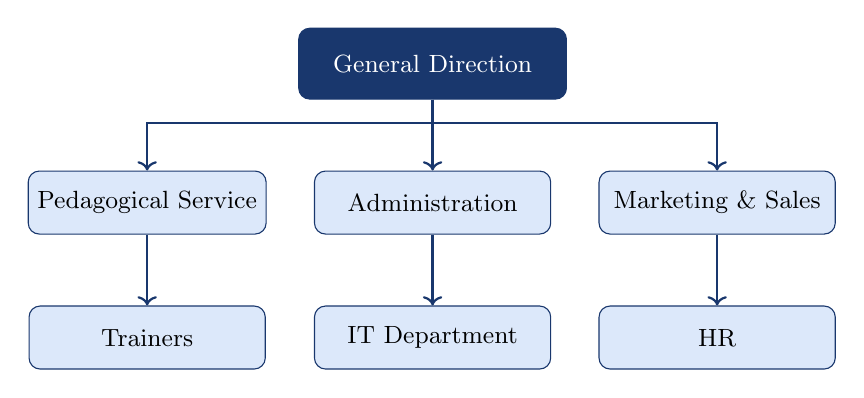
\begin{tikzpicture}[
  node distance=0.9cm and 0.6cm,
  every node/.style={font=\small},
  box/.style={rectangle, draw=primary, fill=softblue, rounded corners=4pt,
              minimum width=3cm, minimum height=0.8cm, align=center},
  topbox/.style={rectangle, draw=primary, fill=primary, text=white,
                 rounded corners=4pt, minimum width=3.4cm, minimum height=0.9cm, align=center}
]
  \node[topbox] (dg) {General Direction};
  \node[box, below=of dg] (admin) {Administration};
  \node[box, left=of admin] (ped) {Pedagogical Service};
  \node[box, right=of admin] (com) {Marketing \& Sales};
  \node[box, below=of ped] (tr) {Trainers};
  \node[box, below=of admin] (it) {IT Department};
  \node[box, below=of com] (rh) {HR};

  \draw[->, thick, color=primary] (dg) -- (admin);
  \draw[->, thick, color=primary] (dg.south) -- ++(0,-0.3) -| (ped.north);
  \draw[->, thick, color=primary] (dg.south) -- ++(0,-0.3) -| (com.north);
  \draw[->, thick, color=primary] (ped) -- (tr);
  \draw[->, thick, color=primary] (admin) -- (it);
  \draw[->, thick, color=primary] (com) -- (rh);
\end{tikzpicture}
\caption{Organizational chart of ADVANCIA Training Center}
\label{fig:orgchart}
\end{figure}

% ---------- 1.3 Project context ----------
\section{Project Context and Problem Statement}

\subsection{Context}

This project takes place within the framework of an end-of-studies internship in computer science, in collaboration between \textbf{ISET Siliana} and \textbf{ADVANCIA Training Center}. It aims at modernizing the way the company handles its trainings and interacts with its users, by replacing manual or scattered processes with a centralized and intelligent web platform.

\subsection{Problem statement}

After studying the company's daily workflow, we identified several recurring difficulties that hinder both the user experience and the administrative efficiency :

\begin{itemize}[leftmargin=2em,itemsep=0.3em]
  \item \textbf{Lack of a unified digital channel :} reservations are taken by phone, e-mail or in person, generating ambiguity and loss of information.
  \item \textbf{Manual user management :} user records and registrations are handled through spreadsheets, which is error-prone and not scalable.
  \item \textbf{No real-time visibility :} the management has no smart dashboard to track users, reservations or revenue.
  \item \textbf{Limited communication :} no automatic notifications when a reservation is accepted, refused or modified.
  \item \textbf{No integrated assistance :} users have no immediate way to ask for help, beyond classical e-mail support.
\end{itemize}

\subsection{Synthetic statistics on the existing situation}

To quantify the problem, we conducted a small internal survey within the host company. The chart below summarizes the main pain points reported by the staff.

\begin{figure}[H]
\centering
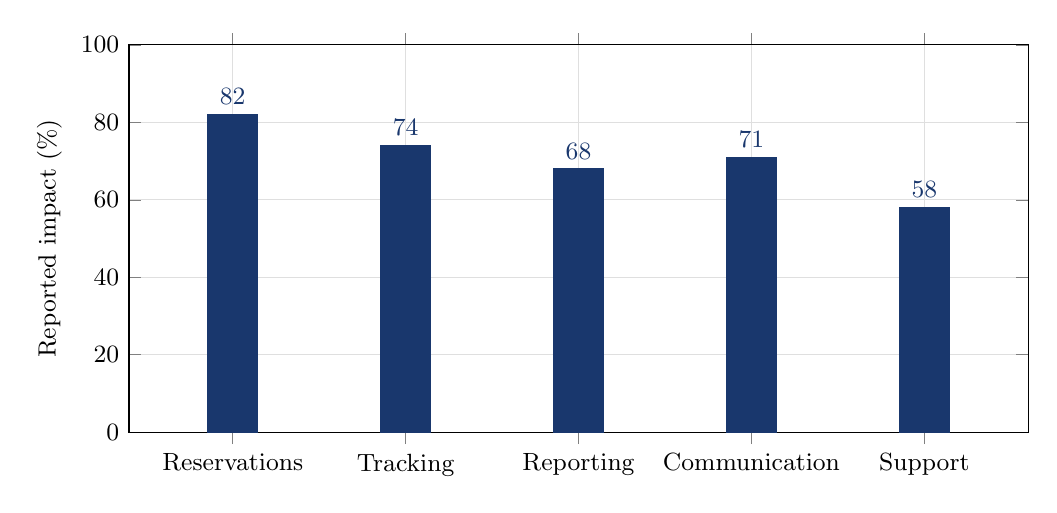
\begin{tikzpicture}
\begin{axis}[
  ybar,
  bar width=18pt,
  width=13cm,
  height=6.5cm,
  ylabel={Reported impact (\%)},
  symbolic x coords={Reservations, Tracking, Reporting, Communication, Support},
  xtick=data,
  ymin=0, ymax=100,
  enlarge x limits=0.15,
  nodes near coords,
  nodes near coords style={font=\small\bfseries, color=primary},
  every axis label/.append style={font=\small},
  tick label style={font=\small},
  legend pos=north east,
  grid=both,
  major grid style={color=gray!25},
  minor grid style={color=gray!10}
]
  \addplot[fill=primary, draw=primary] coordinates {
    (Reservations,82) (Tracking,74) (Reporting,68) (Communication,71) (Support,58)
  };
\end{axis}
\end{tikzpicture}
\caption{Pain points reported by the staff (internal survey, n = 12)}
\label{fig:painpoints}
\end{figure}

% ---------- 1.4 Existing solutions ----------
\section{Study of the Existing Solutions}

Several training-management platforms exist on the market. We compared three of the most representative ones to identify what is missing and what we can do better.

\begin{table}[H]
\centering
\renewcommand{\arraystretch}{1.35}
\begin{tabularx}{\textwidth}{|>{\columncolor{softblue}}l|X|X|X|}
\hline
\rowcolor{primary}
\textbf{\color{white} Criteria} & \textbf{\color{white} Moodle} & \textbf{\color{white} Udemy Business} & \textbf{\color{white} Coursera}\\
\hline
Multi-actor management & Partial & Limited & Limited \\\hline
Smart dashboard / KPIs & No & Partial & Partial \\\hline
Integrated chatbot & No & No & No \\\hline
Reservation workflow & No & No & No \\\hline
Excel / PDF export & Partial & No & No \\\hline
Local deployment cost & Free / Self-hosted & Paid & Paid \\\hline
\end{tabularx}
\caption{Comparative study of existing solutions}
\label{tab:existing}
\end{table}

\subsection{Critique}

The studied platforms are powerful for content delivery, but they remain generic. None of them provides a complete \textit{four-actor reservation workflow}, a \textit{smart dashboard with chatbot} and a \textit{multi-format export} (Excel/PDF) tailored for a Tunisian training center.

% ---------- 1.5 Proposed solution ----------
\section{Proposed Solution}

We propose \textbf{ADVANCIA}, a smart, secure and responsive web platform that brings together every actor of the training process inside one ecosystem. The figure below summarizes the high-level functional architecture of the proposed solution.

\begin{figure}[H]
\centering
\begin{tikzpicture}[
  every node/.style={font=\small},
  actor/.style={rectangle, draw=primary, fill=softblue, rounded corners=4pt,
                minimum width=2.4cm, minimum height=0.9cm, align=center},
  core/.style={ellipse, draw=primary, fill=primary, text=white,
               minimum width=4cm, minimum height=2cm, align=center},
  module/.style={rectangle, draw=secondary, fill=white, rounded corners=4pt,
                 minimum width=2.6cm, minimum height=0.7cm, align=center}
]
  \node[core] (advancia) {\textbf{ADVANCIA}\\Platform};

  \node[actor, above left=1.8cm and 2.6cm of advancia] (user) {\faUser\ User};
  \node[actor, above right=1.8cm and 2.6cm of advancia] (trainer) {\faChalkboardTeacher\ Trainer};
  \node[actor, below left=1.8cm and 2.6cm of advancia] (admin) {\faUserShield\ Admin};
  \node[actor, below right=1.8cm and 2.6cm of advancia] (super) {\faUserCog\ Super-Admin};

  \draw[->, thick, primary] (user) -- (advancia);
  \draw[->, thick, primary] (trainer) -- (advancia);
  \draw[->, thick, primary] (admin) -- (advancia);
  \draw[->, thick, primary] (super) -- (advancia);

  \node[module, right=4.2cm of advancia] (mod1) {Catalog};
  \node[module, below=0.2cm of mod1] (mod2) {Reservations};
  \node[module, below=0.2cm of mod2] (mod3) {Dashboard};
  \node[module, below=0.2cm of mod3] (mod4) {Chatbot};
  \node[module, below=0.2cm of mod4] (mod5) {Notifications};

  \draw[->, dashed, secondary] (advancia.east) -- (mod1.west);
  \draw[->, dashed, secondary] (advancia.east) -- (mod2.west);
  \draw[->, dashed, secondary] (advancia.east) -- (mod3.west);
  \draw[->, dashed, secondary] (advancia.east) -- (mod4.west);
  \draw[->, dashed, secondary] (advancia.east) -- (mod5.west);
\end{tikzpicture}
\caption{High-level overview of the ADVANCIA platform}
\label{fig:advancia}
\end{figure}

% ---------- 1.6 Methodology ----------
\section{Adopted Methodology : Scrum}

\subsection{Why agile ?}

The functional perimeter of \textit{ADVANCIA} is broad and the requirements are likely to evolve. A \textbf{rigid waterfall} approach would have led to a tunnel effect : a long phase of specification, then a long development, then a single deliverable -- with all the risks that this implies. We therefore chose the \textbf{Scrum} agile framework, which is iterative, incremental and oriented around tangible value at the end of each cycle.

\subsection{Scrum overview}

\begin{figure}[H]
\centering
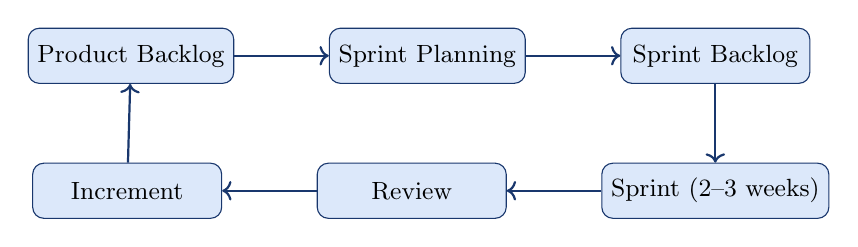
\begin{tikzpicture}[
  every node/.style={font=\small},
  bb/.style={rectangle, draw=primary, fill=softblue, rounded corners=4pt,
             minimum width=2.4cm, minimum height=0.7cm, align=center},
  arrowstyle/.style={->, thick, color=primary}
]
  \node[bb] (pb) {Product Backlog};
  \node[bb, right=1.2cm of pb] (sp) {Sprint Planning};
  \node[bb, right=1.2cm of sp] (sb) {Sprint Backlog};
  \node[bb, below=1.0cm of sb] (sprint) {Sprint (2--3 weeks)};
  \node[bb, left=1.2cm of sprint] (review) {Review};
  \node[bb, left=1.2cm of review] (inc) {Increment};

  \draw[arrowstyle] (pb) -- (sp);
  \draw[arrowstyle] (sp) -- (sb);
  \draw[arrowstyle] (sb) -- (sprint);
  \draw[arrowstyle] (sprint) -- (review);
  \draw[arrowstyle] (review) -- (inc);
  \draw[arrowstyle] (inc) -- (pb);
\end{tikzpicture}
\caption{The Scrum cycle adopted in this project}
\label{fig:scrum}
\end{figure}

\subsection{Scrum roles in our project}

\begin{table}[H]
\centering
\renewcommand{\arraystretch}{1.3}
\begin{tabularx}{\textwidth}{|>{\columncolor{softblue}}l|X|}
\hline
\rowcolor{primary}
\textbf{\color{white} Role} & \textbf{\color{white} Holder \& mission}\\
\hline
Product Owner & Professional supervisor at ADVANCIA -- defines the vision and prioritizes the backlog. \\\hline
Scrum Master & Academic supervisor at ISET Siliana -- enforces the process and removes blockers. \\\hline
Development Team & Istabrak BEN KHMAYS \& Sayhi MAHDI -- design, develop, test and deliver the increments. \\\hline
\end{tabularx}
\caption{Scrum roles in the ADVANCIA project}
\label{tab:scrumroles}
\end{table}

% ---------- Conclusion ----------
\section{Conclusion}

This first chapter has settled the foundations of our work : the host company, the context, the limits of existing solutions, the proposed platform and the agile process that will drive the implementation. The next chapter goes deeper, by capturing the full set of requirements and by translating them into a structured plan of releases and sprints.
     % Project Framework Presentation
% =============================================================
%  CHAPTER 2 - ANALYSIS & PROJECT PLANNING
% =============================================================

\chapteroverview{Analysis and Project Planning}{
  \item Introduction
  \item Identification of the Actors
  \item Functional Requirements
  \item Non-Functional Requirements
  \item Global Use Case Diagram
  \item Product Backlog
  \item Releases and Sprints
  \item Provisional Schedule (Gantt)
  \item Conclusion
}

\section{Introduction}

After framing the project, this chapter focuses on understanding \textit{what} the ADVANCIA platform must do and \textit{how} the work is organized. We start by identifying every actor of the system, we then formalize the functional and non-functional requirements, we draw the global use case diagram and finally we transform the whole into a structured plan of releases, sprints and a Gantt schedule.

% ---------- 2.2 Actors ----------
\section{Identification of the Actors}

The ADVANCIA platform is a multi-actor system. Four main actors interact with the system, each one with a clearly defined scope of responsibilities.

\begin{table}[H]
\centering
\renewcommand{\arraystretch}{1.35}
\begin{tabularx}{\textwidth}{|>{\columncolor{softblue}}l|X|}
\hline
\rowcolor{primary}
\textbf{\color{white} Actor} & \textbf{\color{white} Role and responsibilities}\\
\hline
\textbf{User} &
Creates and manages his account, browses and reserves trainings, manages his profile (photo, avatar, password) and consults his personal dashboard. \\\hline
\textbf{Trainer} &
Handles the trainings he is responsible for, follows enrolled users, animates sessions and updates pedagogical content. \\\hline
\textbf{Administrator} &
Manages users, validates or refuses reservations, imports and exports data (Excel, PDF), exploits a smart dashboard and an integrated chatbot. \\\hline
\textbf{Super-Administrator} &
Has the highest level of authority : manages users, admins, trainers, trainings and courses, sends notifications and supervises the whole platform. \\\hline
\end{tabularx}
\caption{Actors of the ADVANCIA platform}
\label{tab:actors}
\end{table}

% ---------- 2.3 Functional ----------
\section{Functional Requirements}

The functional requirements describe \textit{what} the system must offer. They are grouped by actor.

\subsection{User}
\begin{itemize}[leftmargin=2em,itemsep=0.2em]
  \item Create an account and authenticate.
  \item Manage the personal profile : photo, avatar, password, contact info.
  \item Browse and search the catalog of trainings.
  \item Reserve a training session.
  \item Consult a simple personal dashboard with the essential indicators.
  \item Receive notifications about reservations and account events.
\end{itemize}

\subsection{Trainer}
\begin{itemize}[leftmargin=2em,itemsep=0.2em]
  \item Authenticate and manage profile.
  \item Consult the list of trainings and sessions assigned to him.
  \item Track enrolled users.
  \item Update pedagogical resources of his courses.
\end{itemize}

\subsection{Administrator}
\begin{itemize}[leftmargin=2em,itemsep=0.2em]
  \item Manage users (create, update, suspend, delete).
  \item Import data (e.g. CSV/Excel of users) and export data in Excel or PDF.
  \item Use the smart dashboard with KPIs and charts.
  \item Use the integrated chatbot for assistance and quick queries.
  \item Manage personal profile.
\end{itemize}

\subsection{Super-Administrator}
\begin{itemize}[leftmargin=2em,itemsep=0.2em]
  \item All capabilities of the Administrator.
  \item Manage admins and trainers.
  \item Manage trainings and courses (CRUD).
  \item Accept or refuse reservations.
  \item Send notifications to users or administrators.
  \item Change password and supervise security policies.
\end{itemize}

% ---------- 2.4 Non functional ----------
\section{Non-Functional Requirements}

\begin{table}[H]
\centering
\renewcommand{\arraystretch}{1.35}
\begin{tabularx}{\textwidth}{|>{\columncolor{softblue}}l|X|}
\hline
\rowcolor{primary}
\textbf{\color{white} Requirement} & \textbf{\color{white} Description}\\
\hline
Security & Authentication via JWT, password hashing, role-based access control, HTTPS. \\\hline
Performance & Response time below 2 seconds for the main pages, smooth navigation. \\\hline
Usability & Modern, clear and responsive UI accessible from desktop, tablet and mobile. \\\hline
Reliability & Daily database backup and graceful error handling. \\\hline
Scalability & Modular architecture allowing the addition of new modules without disruption. \\\hline
Maintainability & Clean code, documented modules, version-controlled with Git. \\\hline
Portability & Cross-browser compatibility (Chrome, Firefox, Edge). \\\hline
\end{tabularx}
\caption{Non-functional requirements}
\label{tab:nonfunctional}
\end{table}

% ---------- 2.5 Use case diagram ----------
\section{Global Use Case Diagram}

The following diagram synthesizes the main use cases of the ADVANCIA platform and the relationships between actors and use cases.

\begin{figure}[H]
\centering
\resizebox{\textwidth}{!}{%
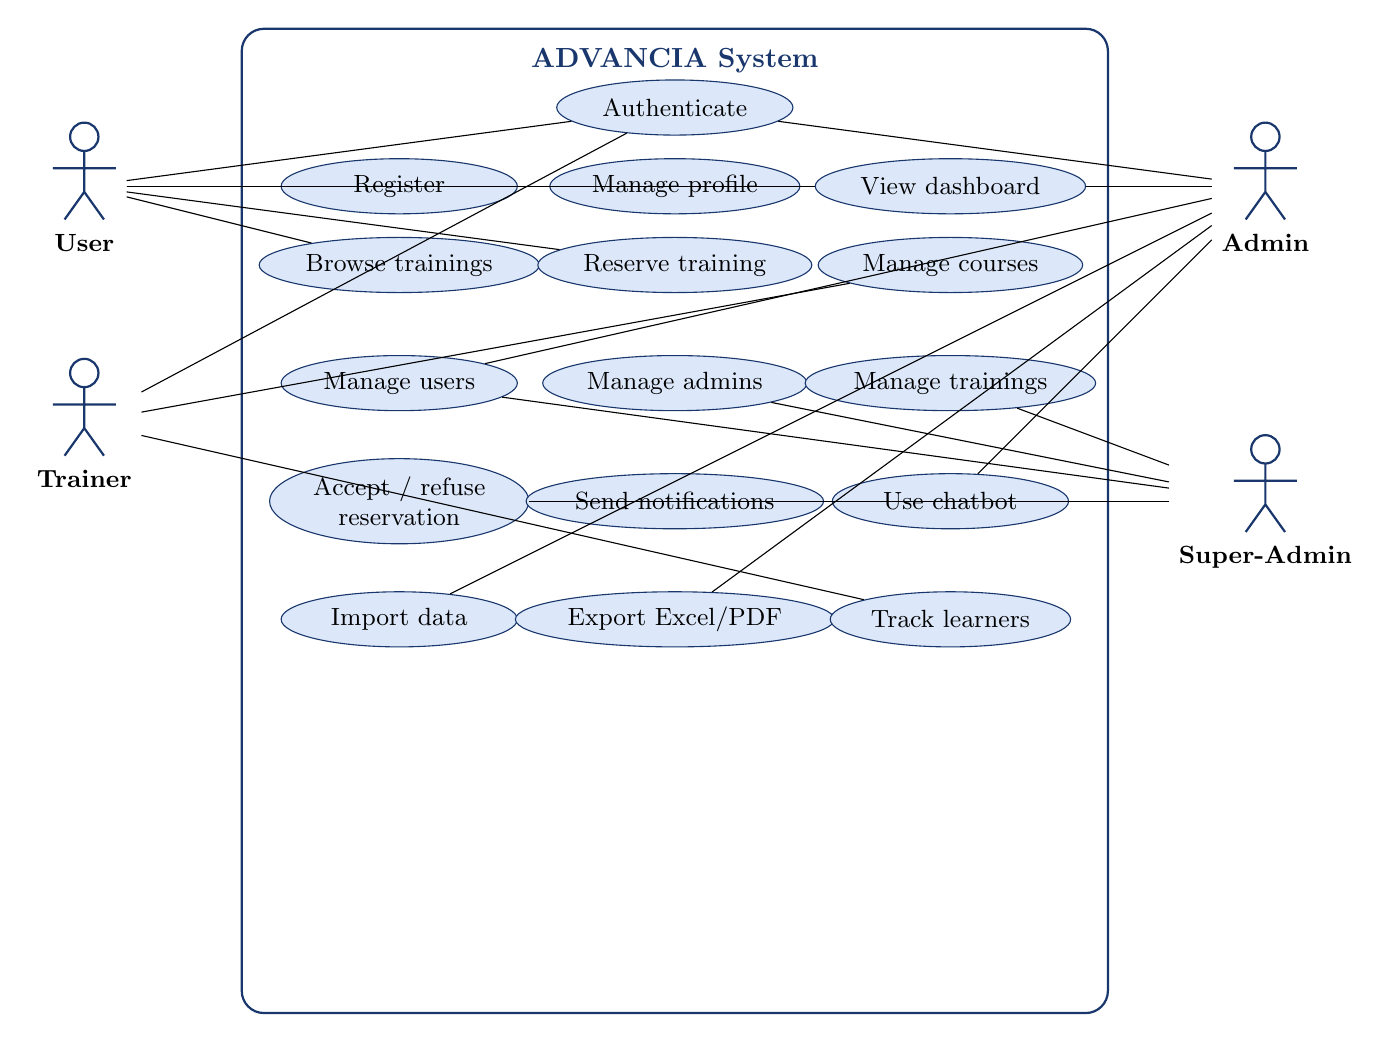
\begin{tikzpicture}[
  every node/.style={font=\small},
  uc/.style={ellipse, draw=primary, fill=softblue, minimum width=3cm,
             minimum height=0.7cm, align=center, inner sep=2pt},
  actor/.style={align=center, font=\small\bfseries}
]
  % System boundary
  \draw[draw=primary, thick, rounded corners=8pt] (-1,-7.5) rectangle (10,5);
  \node[font=\bfseries\color{primary}] at (4.5,4.6) {ADVANCIA System};

  % Use cases
  \node[uc] (auth)   at (4.5, 4)  {Authenticate};
  \node[uc] (regis)  at (1.0, 3)  {Register};
  \node[uc] (profile)at (4.5, 3)  {Manage profile};
  \node[uc] (browse) at (1.0, 2)  {Browse trainings};
  \node[uc] (reserve)at (4.5, 2)  {Reserve training};
  \node[uc] (dash)   at (8.0, 3)  {View dashboard};
  \node[uc] (course) at (8.0, 2)  {Manage courses};
  \node[uc] (mu)     at (1.0, 0.5){Manage users};
  \node[uc] (ma)     at (4.5, 0.5){Manage admins};
  \node[uc] (mt)     at (8.0, 0.5){Manage trainings};
  \node[uc] (accept) at (1.0,-1)  {Accept / refuse\\reservation};
  \node[uc] (notif)  at (4.5,-1)  {Send notifications};
  \node[uc] (chat)   at (8.0,-1)  {Use chatbot};
  \node[uc] (imp)    at (1.0,-2.5){Import data};
  \node[uc] (exp)    at (4.5,-2.5){Export Excel/PDF};
  \node[uc] (track)  at (8.0,-2.5){Track learners};

  % Actors (left: User, Trainer)
  \node[actor] (user) at (-3,3)
       {\tikz\draw[primary, thick] (0,0) circle (0.18) (0,-0.18) -- (0,-0.7)
         (-0.4,-0.4) -- (0.4,-0.4) (-0.25,-1.05) -- (0,-0.7) -- (0.25,-1.05);\\User};
  \node[actor] (trainer) at (-3,0)
       {\tikz\draw[primary, thick] (0,0) circle (0.18) (0,-0.18) -- (0,-0.7)
         (-0.4,-0.4) -- (0.4,-0.4) (-0.25,-1.05) -- (0,-0.7) -- (0.25,-1.05);\\Trainer};

  % Actors (right: Admin, Super-Admin)
  \node[actor] (admin) at (12,3)
       {\tikz\draw[primary, thick] (0,0) circle (0.18) (0,-0.18) -- (0,-0.7)
         (-0.4,-0.4) -- (0.4,-0.4) (-0.25,-1.05) -- (0,-0.7) -- (0.25,-1.05);\\Admin};
  \node[actor] (super) at (12,-1)
       {\tikz\draw[primary, thick] (0,0) circle (0.18) (0,-0.18) -- (0,-0.7)
         (-0.4,-0.4) -- (0.4,-0.4) (-0.25,-1.05) -- (0,-0.7) -- (0.25,-1.05);\\Super-Admin};

  % Links - User
  \draw (user) -- (auth);
  \draw (user) -- (regis);
  \draw (user) -- (profile);
  \draw (user) -- (browse);
  \draw (user) -- (reserve);
  \draw (user) -- (dash);

  % Links - Trainer
  \draw (trainer) -- (auth);
  \draw (trainer) -- (course);
  \draw (trainer) -- (track);

  % Links - Admin
  \draw (admin) -- (auth);
  \draw (admin) -- (mu);
  \draw (admin) -- (dash);
  \draw (admin) -- (chat);
  \draw (admin) -- (imp);
  \draw (admin) -- (exp);

  % Links - Super-Admin
  \draw (super) -- (mu);
  \draw (super) -- (ma);
  \draw (super) -- (mt);
  \draw (super) -- (accept);
  \draw (super) -- (notif);
  \draw (super) -- (chat);
\end{tikzpicture}}
\caption{Global use case diagram of the ADVANCIA platform}
\label{fig:globaluc}
\end{figure}

% ---------- 2.6 Product Backlog ----------
\section{Product Backlog}

The product backlog gathers, in priority order, every user story to be developed. The story points (SP) follow a Fibonacci scale.

\begin{longtable}{|>{\columncolor{softblue}}p{0.9cm}|p{8.5cm}|p{2.3cm}|p{1.1cm}|}
\hline
\rowcolor{primary}
\textbf{\color{white} ID} & \textbf{\color{white} User Story} & \textbf{\color{white} Actor} & \textbf{\color{white} SP}\\
\hline
\endfirsthead
\hline
\rowcolor{primary}
\textbf{\color{white} ID} & \textbf{\color{white} User Story} & \textbf{\color{white} Actor} & \textbf{\color{white} SP}\\
\hline
\endhead
US01 & As a user, I want to create an account so I can access the platform. & User & 3 \\\hline
US02 & As a user, I want to authenticate securely. & User & 3 \\\hline
US03 & As a user, I want to manage my profile (photo, avatar, password). & User & 5 \\\hline
US04 & As a user, I want a personal dashboard. & User & 5 \\\hline
US05 & As a user, I want to browse and search trainings. & User & 5 \\\hline
US06 & As a user, I want to reserve a training session. & User & 5 \\\hline
US07 & As a trainer, I want to consult my assigned trainings. & Trainer & 3 \\\hline
US08 & As a trainer, I want to track my enrolled learners. & Trainer & 5 \\\hline
US09 & As an admin, I want to manage users (CRUD). & Admin & 8 \\\hline
US10 & As an admin, I want to import data from Excel. & Admin & 5 \\\hline
US11 & As an admin, I want to export data to Excel and PDF. & Admin & 5 \\\hline
US12 & As an admin, I want a smart dashboard. & Admin & 8 \\\hline
US13 & As an admin, I want an integrated chatbot. & Admin & 8 \\\hline
US14 & As a super-admin, I want to manage admins and trainers. & Super-Admin & 8 \\\hline
US15 & As a super-admin, I want to manage trainings and courses. & Super-Admin & 8 \\\hline
US16 & As a super-admin, I want to accept or refuse reservations. & Super-Admin & 5 \\\hline
US17 & As a super-admin, I want to send notifications. & Super-Admin & 5 \\\hline
US18 & As any actor, I want a responsive and modern UI. & All & 5 \\\hline
\caption{Product backlog of the ADVANCIA platform}
\label{tab:backlog}
\end{longtable}

% ---------- 2.7 Releases and sprints ----------
\section{Releases and Sprints}

The product backlog has been broken down into \textbf{three releases}, each one delivering a tangible set of value at the end of its lifecycle.

\begin{table}[H]
\centering
\renewcommand{\arraystretch}{1.35}
\begin{tabularx}{\textwidth}{|>{\columncolor{softblue}}l|X|l|}
\hline
\rowcolor{primary}
\textbf{\color{white} Release} & \textbf{\color{white} Scope} & \textbf{\color{white} Sprints}\\
\hline
Release 1 & Authentication \& User management (US01--US04, US18) & S1, S2 \\\hline
Release 2 & Training catalog \& Course management (US05, US07, US15) & S3, S4 \\\hline
Release 3 & Reservation, Notifications, Dashboard \& Chatbot (US06, US08--US14, US16, US17) & S5, S6 \\\hline
\end{tabularx}
\caption{Decomposition into releases and sprints}
\label{tab:releases}
\end{table}

\subsection{Distribution of effort}

\begin{figure}[H]
\centering
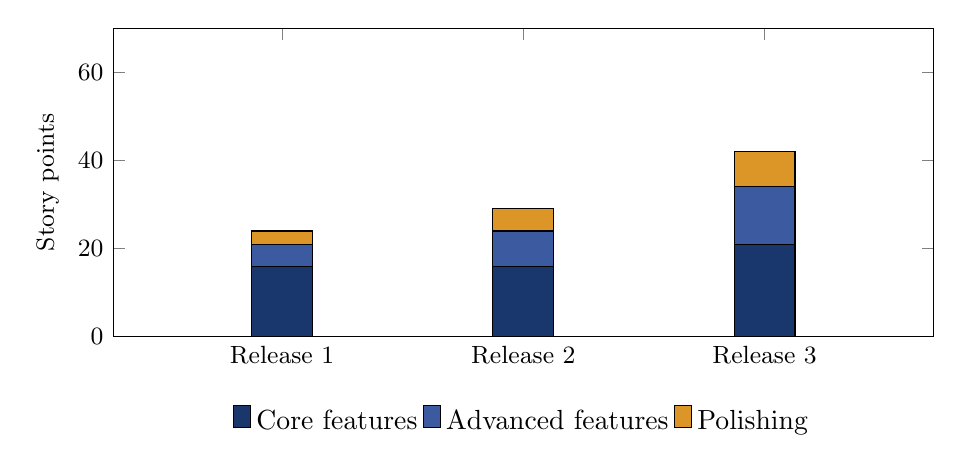
\begin{tikzpicture}
\begin{axis}[
  width=12cm, height=5.5cm,
  ybar stacked,
  bar width=22pt,
  ylabel={Story points},
  symbolic x coords={Release 1, Release 2, Release 3},
  xtick=data,
  ymin=0, ymax=70,
  legend style={at={(0.5,-0.20)}, anchor=north, legend columns=-1, draw=none},
  enlarge x limits=0.35,
  nodes near coords style={font=\small\color{white}\bfseries},
  every axis label/.append style={font=\small},
  tick label style={font=\small}
]
  \addplot[fill=primary]    coordinates {(Release 1,16) (Release 2,16) (Release 3,21)};
  \addplot[fill=secondary]  coordinates {(Release 1,5)  (Release 2,8)  (Release 3,13)};
  \addplot[fill=accent]     coordinates {(Release 1,3)  (Release 2,5)  (Release 3,8) };
  \legend{Core features, Advanced features, Polishing}
\end{axis}
\end{tikzpicture}
\caption{Distribution of story points across releases}
\label{fig:effort}
\end{figure}

% ---------- 2.8 Gantt ----------
\section{Provisional Schedule (Gantt Chart)}

\begin{figure}[H]
\centering
\resizebox{\textwidth}{!}{%
\begin{ganttchart}[
  hgrid, vgrid,
  bar/.append style={fill=primary, draw=primary},
  bar incomplete/.append style={fill=softblue, draw=primary},
  group/.append style={fill=secondary, draw=secondary},
  milestone/.append style={fill=accent, draw=accent},
  bar height=0.6,
  group label font=\bfseries\color{white},
  bar label font=\small,
  title label font=\bfseries\color{primary},
  title height=1,
  x unit=0.55cm,
  y unit chart=0.55cm
]{1}{20}
  \gantttitle{ADVANCIA Project -- Provisional Planning}{20} \\
  \gantttitlelist{1,...,20}{1} \\
  \ganttgroup{Analysis \& Design}{1}{4} \\
  \ganttbar{Requirements}{1}{2} \\
  \ganttbar{UML modeling}{2}{4} \\
  \ganttgroup{Release 1}{4}{8} \\
  \ganttbar{Sprint 1 -- Auth}{4}{6} \\
  \ganttbar{Sprint 2 -- User mgmt}{6}{8} \\
  \ganttgroup{Release 2}{8}{13} \\
  \ganttbar{Sprint 3 -- Catalog}{8}{10} \\
  \ganttbar{Sprint 4 -- Courses}{11}{13} \\
  \ganttgroup{Release 3}{13}{18} \\
  \ganttbar{Sprint 5 -- Reservations}{13}{15} \\
  \ganttbar{Sprint 6 -- Dashboard \& Chatbot}{16}{18} \\
  \ganttgroup{Tests \& Documentation}{18}{20} \\
  \ganttbar{Final tests}{18}{19} \\
  \ganttbar{Documentation}{19}{20} \\
  \ganttmilestone{Final delivery}{20}
\end{ganttchart}}
\caption{Gantt chart of the ADVANCIA project}
\label{fig:gantt}
\end{figure}

\section{Conclusion}

This second chapter has clarified the perimeter of the platform : its four actors, its functional and non-functional requirements, the global use cases, and the structuring of the work into three releases driven by a Gantt schedule. The next chapters will detail each release, sprint by sprint, until the final integrated solution.
     % Analysis & Project Planning
% =============================================================
%  CHAPTER 3 - RELEASE 1 : AUTHENTICATION & USER MANAGEMENT
% =============================================================

\chapteroverview{Release 1 : Authentication \& User Management}{
  \item Introduction
  \item Sprint Backlog
  \item Refined Use Cases
  \item Sequence Diagrams
  \item Class Diagram of the Module
  \item Achieved Increment
  \item Conclusion
}

\section{Introduction}

The first release lays the security foundations of the platform. It delivers everything that revolves around \textit{identity} : registration, secure authentication, profile management and the personal user dashboard. Without this layer, no other module can be safely built on top.

% ---------- 3.2 Sprint backlog ----------
\section{Sprint Backlog}

\begin{table}[H]
\centering
\renewcommand{\arraystretch}{1.35}
\begin{tabularx}{\textwidth}{|>{\columncolor{softblue}}c|X|c|c|}
\hline
\rowcolor{primary}
\textbf{\color{white} ID} & \textbf{\color{white} Task} & \textbf{\color{white} Sprint} & \textbf{\color{white} Status}\\
\hline
T1 & Database design (users, roles, sessions) & S1 & \checkmark \\\hline
T2 & Sign-up form with field validation & S1 & \checkmark \\\hline
T3 & Login with JWT \& password hashing & S1 & \checkmark \\\hline
T4 & Forgot / reset password & S1 & \checkmark \\\hline
T5 & User profile : photo \& avatar upload & S2 & \checkmark \\\hline
T6 & Change password from profile & S2 & \checkmark \\\hline
T7 & Personal dashboard widgets & S2 & \checkmark \\\hline
T8 & Role-based access middleware & S2 & \checkmark \\\hline
\end{tabularx}
\caption{Sprint backlog -- Release 1}
\label{tab:sb1}
\end{table}

% ---------- 3.3 Use cases ----------
\section{Refined Use Cases}

\subsection{Detailed use case : \textit{Sign-up}}

\begin{table}[H]
\centering
\renewcommand{\arraystretch}{1.3}
\begin{tabularx}{\textwidth}{|>{\columncolor{softblue}}p{3.5cm}|X|}
\hline
\textbf{Title}        & Sign-up \\\hline
\textbf{Actor}        & User \\\hline
\textbf{Goal}         & Create a personal account on the platform. \\\hline
\textbf{Pre-condition}& The user is not yet registered. \\\hline
\textbf{Main scenario}& 1. The user opens the sign-up page. \newline
                        2. The system displays the form. \newline
                        3. The user fills in the required fields. \newline
                        4. The system validates the data. \newline
                        5. The system creates the account and sends a confirmation. \\\hline
\textbf{Alternative}  & 4.a If the e-mail already exists, the system displays an error. \\\hline
\textbf{Post-condition}& The account is created and ready to be activated. \\\hline
\end{tabularx}
\caption{Detailed use case : Sign-up}
\label{tab:uc-signup}
\end{table}

\subsection{Use case diagram of Release 1}

\begin{figure}[H]
\centering
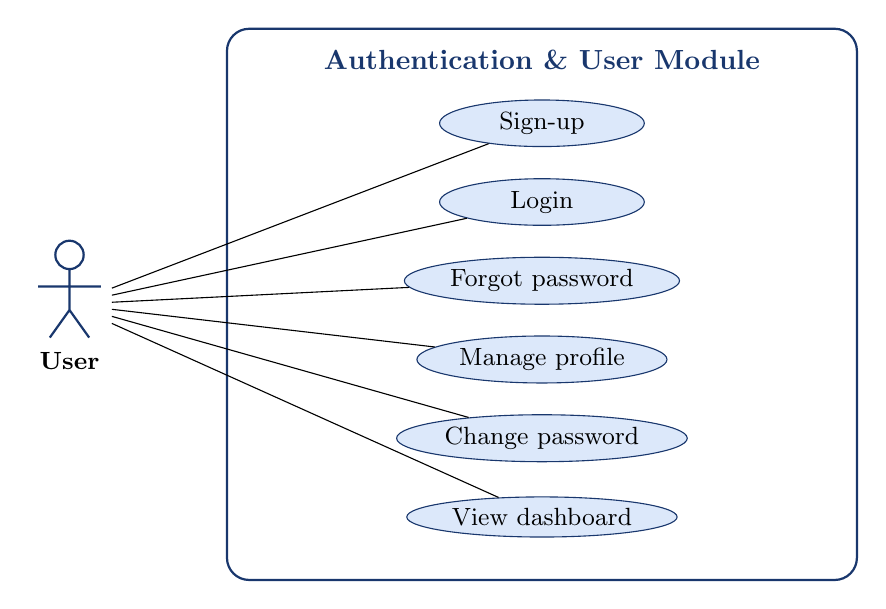
\begin{tikzpicture}[
  every node/.style={font=\small},
  uc/.style={ellipse, draw=primary, fill=softblue, minimum width=2.6cm, align=center, inner sep=2pt}
]
  \draw[draw=primary, thick, rounded corners=8pt] (0,-3.5) rectangle (8,3.5);
  \node[font=\bfseries\color{primary}] at (4,3.1) {Authentication \& User Module};

  \node[uc] (su) at (4,2.3) {Sign-up};
  \node[uc] (lo) at (4,1.3) {Login};
  \node[uc] (fp) at (4,0.3) {Forgot password};
  \node[uc] (mp) at (4,-0.7) {Manage profile};
  \node[uc] (cp) at (4,-1.7) {Change password};
  \node[uc] (db) at (4,-2.7) {View dashboard};

  \node[align=center] (user) at (-2,0)
       {\tikz\draw[primary, thick] (0,0) circle (0.18) (0,-0.18) -- (0,-0.7)
         (-0.4,-0.4) -- (0.4,-0.4) (-0.25,-1.05) -- (0,-0.7) -- (0.25,-1.05);\\\textbf{User}};

  \draw (user) -- (su);
  \draw (user) -- (lo);
  \draw (user) -- (fp);
  \draw (user) -- (mp);
  \draw (user) -- (cp);
  \draw (user) -- (db);
\end{tikzpicture}
\caption{Use case diagram -- Release 1}
\label{fig:uc-r1}
\end{figure}

% ---------- 3.4 Sequence diagrams ----------
\section{Sequence Diagrams}

\subsection{Sequence : Login}

\begin{figure}[H]
\centering
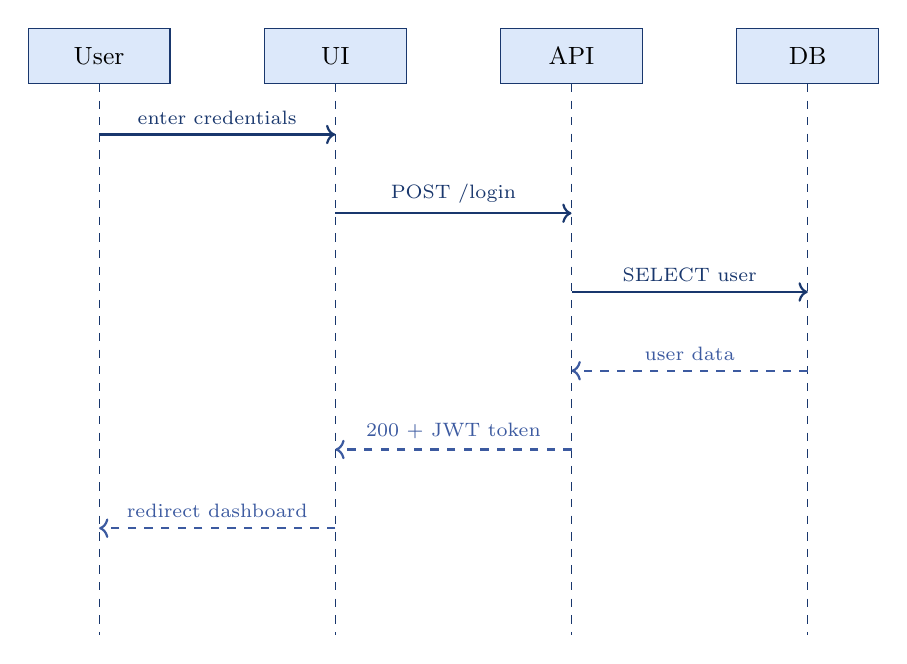
\begin{tikzpicture}[
  every node/.style={font=\small},
  lifeline/.style={dashed, color=primary},
  msg/.style={->, thick, color=primary},
  ret/.style={->, thick, dashed, color=secondary},
  actor/.style={rectangle, draw=primary, fill=softblue, minimum width=1.8cm, minimum height=0.7cm}
]
  \node[actor] (u)  at (0,0)  {User};
  \node[actor] (ui) at (3,0)  {UI};
  \node[actor] (api)at (6,0)  {API};
  \node[actor] (db) at (9,0)  {DB};

  \foreach \n in {u,ui,api,db} \draw[lifeline] (\n.south) -- ++(0,-7);

  \draw[msg] (0,-1)  -- node[above,font=\scriptsize]{enter credentials} (3,-1);
  \draw[msg] (3,-2)  -- node[above,font=\scriptsize]{POST /login} (6,-2);
  \draw[msg] (6,-3)  -- node[above,font=\scriptsize]{SELECT user} (9,-3);
  \draw[ret] (9,-4)  -- node[above,font=\scriptsize]{user data} (6,-4);
  \draw[ret] (6,-5)  -- node[above,font=\scriptsize]{200 + JWT token} (3,-5);
  \draw[ret] (3,-6)  -- node[above,font=\scriptsize]{redirect dashboard} (0,-6);
\end{tikzpicture}
\caption{Sequence diagram of the login process}
\label{fig:sd-login}
\end{figure}

% ---------- 3.5 Class diagram ----------
\section{Class Diagram of the Module}

\begin{figure}[H]
\centering
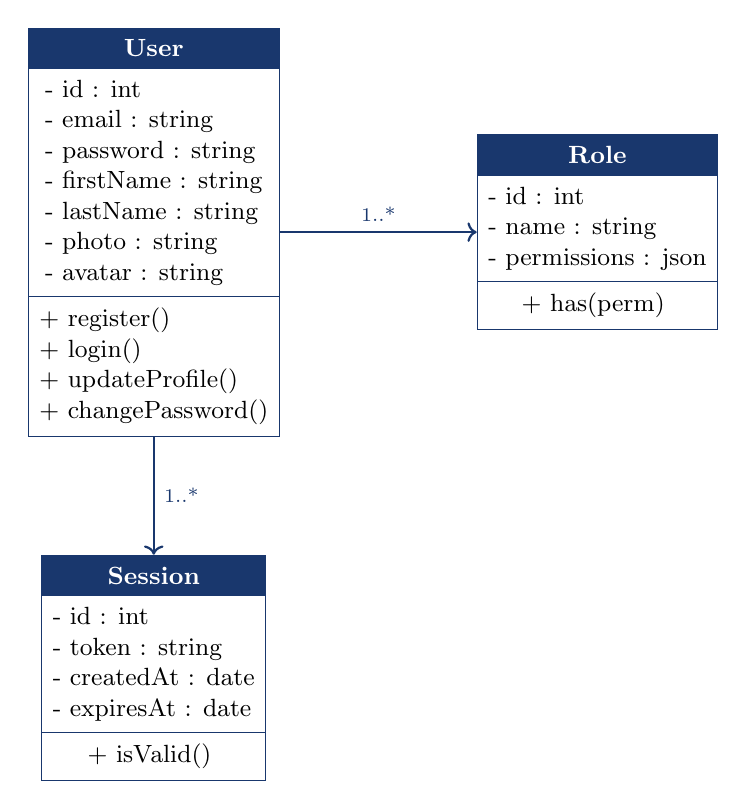
\begin{tikzpicture}[
  every node/.style={font=\small},
  class/.style={rectangle split, rectangle split parts=3, rectangle split part fill={primary, white, white},
                draw=primary, text=white, rectangle split draw splits=true, align=left, inner sep=4pt}
]
  \node[class] (user) at (0,0) {%
    \nodepart{one}\bfseries User
    \nodepart[text=black]{two}
      - id : int\\
      - email : string\\
      - password : string\\
      - firstName : string\\
      - lastName : string\\
      - photo : string\\
      - avatar : string
    \nodepart[text=black]{three}
      + register()\\
      + login()\\
      + updateProfile()\\
      + changePassword()
  };

  \node[class, right=2.5cm of user] (role) {%
    \nodepart{one}\bfseries Role
    \nodepart[text=black]{two}
      - id : int\\
      - name : string\\
      - permissions : json
    \nodepart[text=black]{three}
      + has(perm)
  };

  \node[class, below=1.5cm of user] (session) {%
    \nodepart{one}\bfseries Session
    \nodepart[text=black]{two}
      - id : int\\
      - token : string\\
      - createdAt : date\\
      - expiresAt : date
    \nodepart[text=black]{three}
      + isValid()
  };

  \draw[->, thick, color=primary] (user) -- node[above,font=\scriptsize]{1..*} (role);
  \draw[->, thick, color=primary] (user) -- node[right,font=\scriptsize]{1..*} (session);
\end{tikzpicture}
\caption{Class diagram -- Authentication module}
\label{fig:cd-r1}
\end{figure}

% ---------- 3.6 Achieved increment ----------
\section{Achieved Increment}

At the end of Release 1, the platform delivers :
\begin{itemize}[leftmargin=2em,itemsep=0.2em]
  \item A complete sign-up / login system based on JWT.
  \item Profile management with photo and avatar upload.
  \item Password reset and change.
  \item A first version of the personal dashboard for the user.
  \item A role-based middleware ready to be reused by the next releases.
\end{itemize}

\paragraph{Indicative interfaces.}
The figure below positions, schematically, the screens delivered at the end of this release.

\begin{figure}[H]
\centering
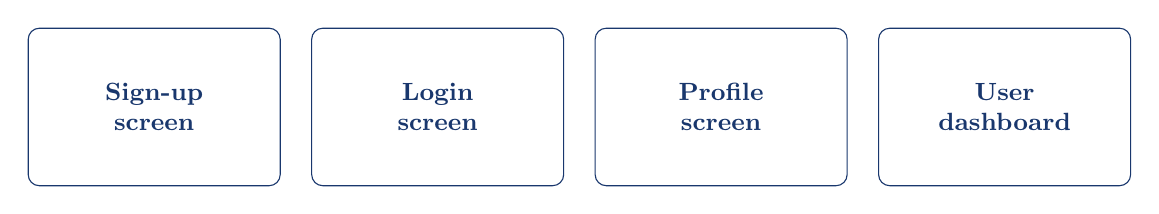
\begin{tikzpicture}[
  scr/.style={rectangle, draw=primary, fill=white, rounded corners=4pt,
              minimum width=3.2cm, minimum height=2.0cm, align=center, font=\small\bfseries\color{primary}}
]
  \node[scr] (a) at (0,0) {Sign-up\\screen};
  \node[scr] (b) at (3.6,0) {Login\\screen};
  \node[scr] (c) at (7.2,0) {Profile\\screen};
  \node[scr] (d) at (10.8,0) {User\\dashboard};
\end{tikzpicture}
\caption{Screens delivered at the end of Release 1}
\label{fig:r1-screens}
\end{figure}

\section{Conclusion}

This first release has stabilized a robust security and identity layer. The next chapter builds on top of it to offer the functional heart of the platform : the training catalog and the course-management module.
     % Release 1 - Authentication & User Management
% =============================================================
%  CHAPTER 4 - RELEASE 2 : TRAINING CATALOG & COURSE MANAGEMENT
% =============================================================

\chapteroverview{Release 2 : Training Catalog \& Course Management}{
  \item Introduction
  \item Sprint Backlog
  \item Refined Use Cases
  \item Sequence Diagrams
  \item Class Diagram of the Module
  \item Achieved Increment
  \item Conclusion
}

\section{Introduction}

The second release shifts the focus from \textit{identity} to \textit{content}. It builds the training catalog browsed by users and the course-management workspace used by trainers and the super-administrator. This is the functional heart of the platform : without trainings, there is nothing to reserve.

% ---------- 4.2 Sprint backlog ----------
\section{Sprint Backlog}

\begin{table}[H]
\centering
\renewcommand{\arraystretch}{1.35}
\begin{tabularx}{\textwidth}{|>{\columncolor{softblue}}c|X|c|c|}
\hline
\rowcolor{primary}
\textbf{\color{white} ID} & \textbf{\color{white} Task} & \textbf{\color{white} Sprint} & \textbf{\color{white} Status}\\
\hline
T9  & DB design (training, course, category, trainer)        & S3 & \checkmark \\\hline
T10 & Public catalog : list, filter, search                  & S3 & \checkmark \\\hline
T11 & Training detail page                                   & S3 & \checkmark \\\hline
T12 & CRUD trainings (super-admin)                           & S4 & \checkmark \\\hline
T13 & CRUD courses inside a training (super-admin / trainer) & S4 & \checkmark \\\hline
T14 & Trainer assignment to a training                       & S4 & \checkmark \\\hline
T15 & Image \& document upload for a course                  & S4 & \checkmark \\\hline
\end{tabularx}
\caption{Sprint backlog -- Release 2}
\label{tab:sb2}
\end{table}

% ---------- 4.3 Use cases ----------
\section{Refined Use Cases}

\subsection{Detailed use case : \textit{Browse trainings}}

\begin{table}[H]
\centering
\renewcommand{\arraystretch}{1.3}
\begin{tabularx}{\textwidth}{|>{\columncolor{softblue}}p{3.5cm}|X|}
\hline
\textbf{Title}        & Browse trainings \\\hline
\textbf{Actor}        & User \\\hline
\textbf{Goal}         & Discover and filter the available trainings. \\\hline
\textbf{Pre-condition}& The user has access to the catalog page. \\\hline
\textbf{Main scenario}& 1. The user opens the catalog. \newline
                        2. The system displays the list of trainings. \newline
                        3. The user filters by category, level or trainer. \newline
                        4. The system updates the result list dynamically. \newline
                        5. The user opens a training to see its detailed page. \\\hline
\textbf{Alternative}  & 2.a If the catalog is empty, the system displays a friendly empty state. \\\hline
\textbf{Post-condition}& The user has all the information needed to decide whether to reserve. \\\hline
\end{tabularx}
\caption{Detailed use case : Browse trainings}
\label{tab:uc-browse}
\end{table}

\subsection{Use case diagram of Release 2}

\begin{figure}[H]
\centering
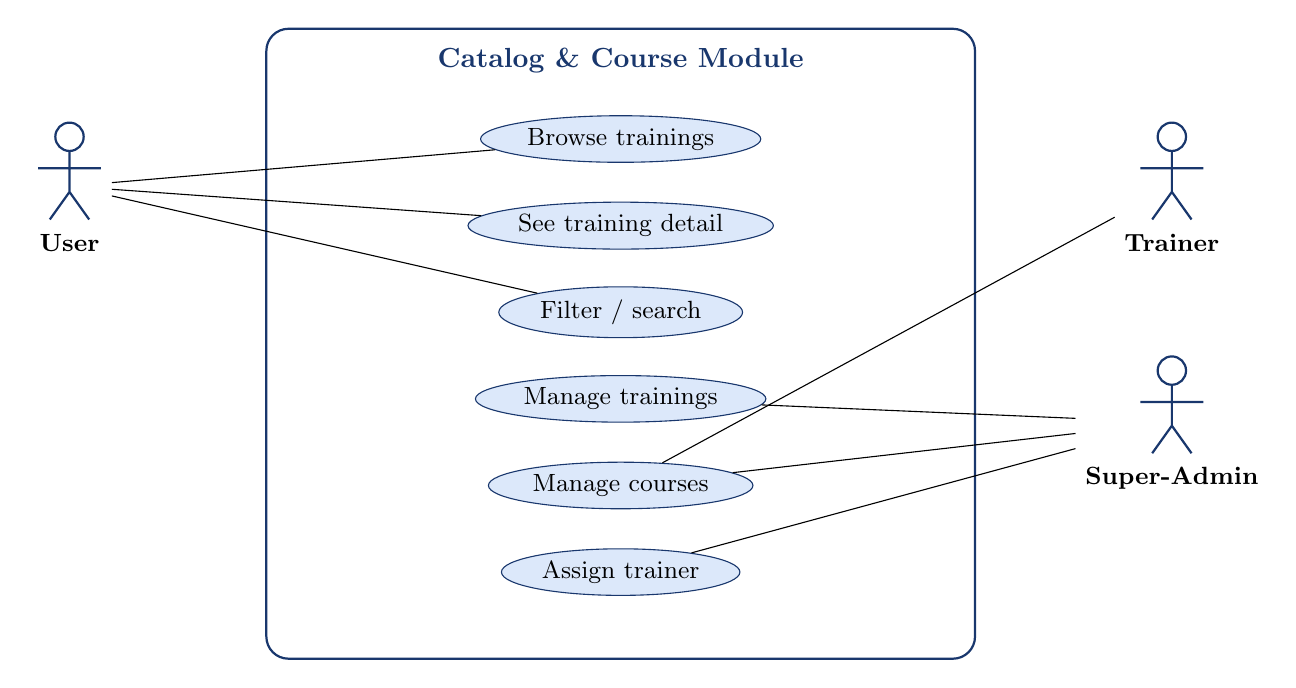
\begin{tikzpicture}[
  every node/.style={font=\small},
  uc/.style={ellipse, draw=primary, fill=softblue, minimum width=2.6cm, align=center, inner sep=2pt}
]
  \draw[draw=primary, thick, rounded corners=8pt] (-0.5,-4) rectangle (8.5,4);
  \node[font=\bfseries\color{primary}] at (4,3.6) {Catalog \& Course Module};

  \node[uc] (browse) at (4, 2.6) {Browse trainings};
  \node[uc] (detail) at (4, 1.5) {See training detail};
  \node[uc] (filter) at (4, 0.4) {Filter / search};
  \node[uc] (mt)     at (4,-0.7) {Manage trainings};
  \node[uc] (mc)     at (4,-1.8) {Manage courses};
  \node[uc] (assign) at (4,-2.9) {Assign trainer};

  \node[align=center] (user) at (-3,2)
       {\tikz\draw[primary, thick] (0,0) circle (0.18) (0,-0.18) -- (0,-0.7)
         (-0.4,-0.4) -- (0.4,-0.4) (-0.25,-1.05) -- (0,-0.7) -- (0.25,-1.05);\\\textbf{User}};

  \node[align=center] (super) at (11,-1)
       {\tikz\draw[primary, thick] (0,0) circle (0.18) (0,-0.18) -- (0,-0.7)
         (-0.4,-0.4) -- (0.4,-0.4) (-0.25,-1.05) -- (0,-0.7) -- (0.25,-1.05);\\\textbf{Super-Admin}};

  \node[align=center] (trainer) at (11,2)
       {\tikz\draw[primary, thick] (0,0) circle (0.18) (0,-0.18) -- (0,-0.7)
         (-0.4,-0.4) -- (0.4,-0.4) (-0.25,-1.05) -- (0,-0.7) -- (0.25,-1.05);\\\textbf{Trainer}};

  \draw (user) -- (browse);
  \draw (user) -- (detail);
  \draw (user) -- (filter);
  \draw (super) -- (mt);
  \draw (super) -- (mc);
  \draw (super) -- (assign);
  \draw (trainer) -- (mc);
\end{tikzpicture}
\caption{Use case diagram -- Release 2}
\label{fig:uc-r2}
\end{figure}

% ---------- 4.4 Sequence diagram ----------
\section{Sequence Diagrams}

\subsection{Sequence : Add a training (super-admin)}

\begin{figure}[H]
\centering
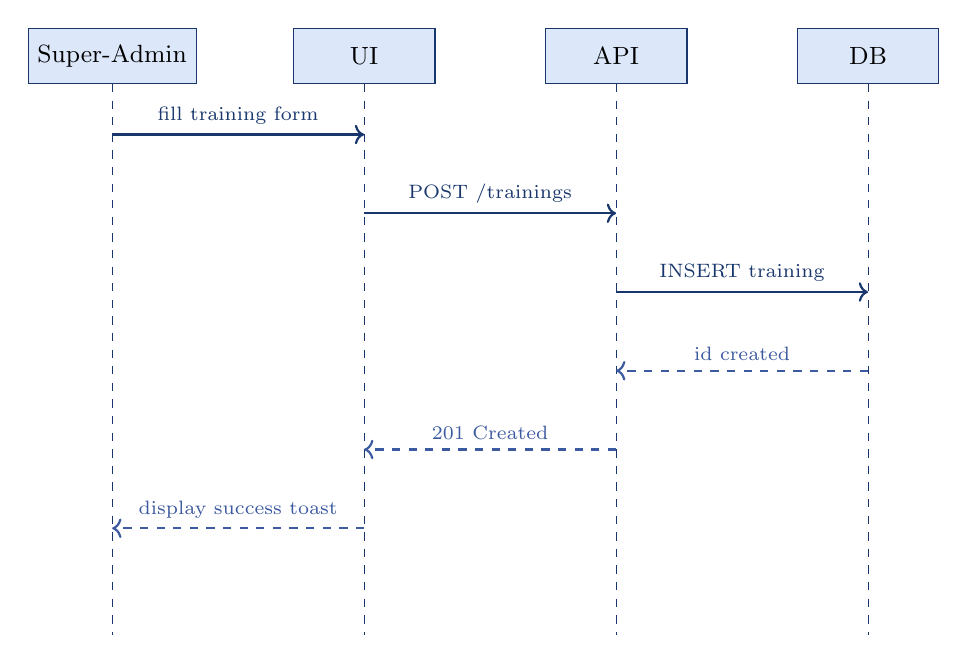
\begin{tikzpicture}[
  every node/.style={font=\small},
  lifeline/.style={dashed, color=primary},
  msg/.style={->, thick, color=primary},
  ret/.style={->, thick, dashed, color=secondary},
  actor/.style={rectangle, draw=primary, fill=softblue, minimum width=1.8cm, minimum height=0.7cm}
]
  \node[actor] (a) at (0,0) {Super-Admin};
  \node[actor] (b) at (3.2,0) {UI};
  \node[actor] (c) at (6.4,0) {API};
  \node[actor] (d) at (9.6,0) {DB};

  \foreach \n in {a,b,c,d} \draw[lifeline] (\n.south) -- ++(0,-7);

  \draw[msg] (0,-1)   -- node[above,font=\scriptsize]{fill training form} (3.2,-1);
  \draw[msg] (3.2,-2) -- node[above,font=\scriptsize]{POST /trainings} (6.4,-2);
  \draw[msg] (6.4,-3) -- node[above,font=\scriptsize]{INSERT training} (9.6,-3);
  \draw[ret] (9.6,-4) -- node[above,font=\scriptsize]{id created} (6.4,-4);
  \draw[ret] (6.4,-5) -- node[above,font=\scriptsize]{201 Created} (3.2,-5);
  \draw[ret] (3.2,-6) -- node[above,font=\scriptsize]{display success toast} (0,-6);
\end{tikzpicture}
\caption{Sequence diagram : Add a training}
\label{fig:sd-addtraining}
\end{figure}

% ---------- 4.5 Class diagram ----------
\section{Class Diagram of the Module}

\begin{figure}[H]
\centering
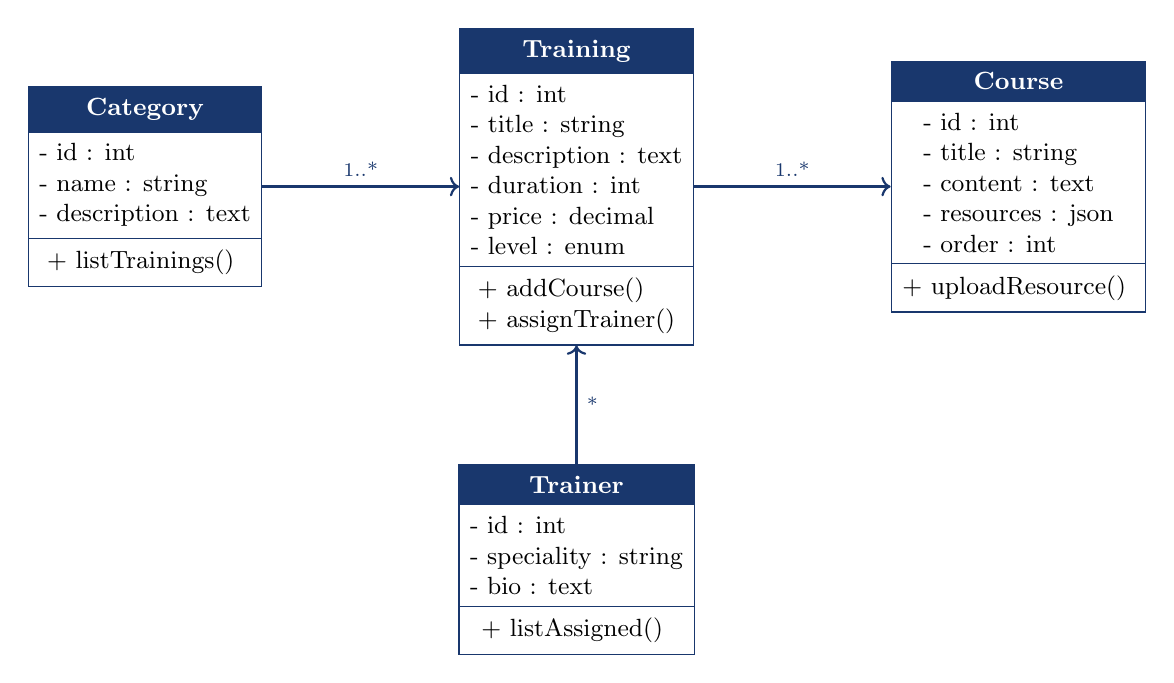
\begin{tikzpicture}[
  every node/.style={font=\small},
  class/.style={rectangle split, rectangle split parts=3,
                rectangle split part fill={primary, white, white},
                draw=primary, text=white, rectangle split draw splits=true, align=left, inner sep=4pt}
]
  \node[class] (cat) at (0,0) {%
    \nodepart{one}\bfseries Category
    \nodepart[text=black]{two}
      - id : int\\
      - name : string\\
      - description : text
    \nodepart[text=black]{three}
      + listTrainings()
  };

  \node[class, right=2.5cm of cat] (tr) {%
    \nodepart{one}\bfseries Training
    \nodepart[text=black]{two}
      - id : int\\
      - title : string\\
      - description : text\\
      - duration : int\\
      - price : decimal\\
      - level : enum
    \nodepart[text=black]{three}
      + addCourse()\\
      + assignTrainer()
  };

  \node[class, right=2.5cm of tr] (course) {%
    \nodepart{one}\bfseries Course
    \nodepart[text=black]{two}
      - id : int\\
      - title : string\\
      - content : text\\
      - resources : json\\
      - order : int
    \nodepart[text=black]{three}
      + uploadResource()
  };

  \node[class, below=1.5cm of tr] (trainer) {%
    \nodepart{one}\bfseries Trainer
    \nodepart[text=black]{two}
      - id : int\\
      - speciality : string\\
      - bio : text
    \nodepart[text=black]{three}
      + listAssigned()
  };

  \draw[->, thick, color=primary] (cat) -- node[above,font=\scriptsize]{1..*} (tr);
  \draw[->, thick, color=primary] (tr) -- node[above,font=\scriptsize]{1..*} (course);
  \draw[->, thick, color=primary] (trainer) -- node[right,font=\scriptsize]{*} (tr);
\end{tikzpicture}
\caption{Class diagram -- Catalog \& Course module}
\label{fig:cd-r2}
\end{figure}

% ---------- 4.6 Increment ----------
\section{Achieved Increment}

\begin{itemize}[leftmargin=2em,itemsep=0.2em]
  \item A public catalog with filter and search.
  \item A detailed page for each training, with the list of its courses.
  \item A super-admin workspace for the full CRUD on trainings, categories and courses.
  \item Trainer assignment, with a dedicated personal area for trainers.
\end{itemize}

\section{Conclusion}

The platform now exposes a real, browsable training catalog backed by a complete administration workspace. The third release will activate the most dynamic part of the system : reservations, notifications, the smart dashboard and the chatbot.
     % Release 2 - Training Catalog & Course Management
% =============================================================
%  CHAPTER 5 - RELEASE 3 : RESERVATION, NOTIFICATIONS, DASHBOARD & CHATBOT
% =============================================================

\chapteroverview{Release 3 : Reservation, Notifications, Dashboard \& Chatbot}{
  \item Introduction
  \item Sprint Backlog
  \item Refined Use Cases
  \item Sequence Diagrams
  \item Class Diagram of the Module
  \item Smart Dashboard \& KPIs
  \item Achieved Increment
  \item Conclusion
}

\section{Introduction}

The third release brings the platform to life. It activates the \textit{reservation} workflow, the \textit{notifications} channel, the \textit{smart dashboard} for the administrators and the \textit{chatbot} that turns the dashboard into a conversational tool. It also closes the import / export feature for Excel and PDF.

% ---------- 5.2 ----------
\section{Sprint Backlog}

\begin{table}[H]
\centering
\renewcommand{\arraystretch}{1.35}
\begin{tabularx}{\textwidth}{|>{\columncolor{softblue}}c|X|c|c|}
\hline
\rowcolor{primary}
\textbf{\color{white} ID} & \textbf{\color{white} Task} & \textbf{\color{white} Sprint} & \textbf{\color{white} Status}\\
\hline
T16 & DB design : reservation, notification        & S5 & \checkmark \\\hline
T17 & Reserve a training (user)                    & S5 & \checkmark \\\hline
T18 & Accept / refuse reservation (super-admin)    & S5 & \checkmark \\\hline
T19 & E-mail \& in-app notifications               & S5 & \checkmark \\\hline
T20 & Smart dashboard : KPIs \& charts             & S6 & \checkmark \\\hline
T21 & Chatbot integration                          & S6 & \checkmark \\\hline
T22 & Import users from Excel                      & S6 & \checkmark \\\hline
T23 & Export data to Excel \& PDF                  & S6 & \checkmark \\\hline
\end{tabularx}
\caption{Sprint backlog -- Release 3}
\label{tab:sb3}
\end{table}

% ---------- 5.3 use cases ----------
\section{Refined Use Cases}

\subsection{Detailed use case : \textit{Reserve a training}}

\begin{table}[H]
\centering
\renewcommand{\arraystretch}{1.3}
\begin{tabularx}{\textwidth}{|>{\columncolor{softblue}}p{3.5cm}|X|}
\hline
\textbf{Title}        & Reserve a training \\\hline
\textbf{Actor}        & User \\\hline
\textbf{Goal}         & Book a seat in an upcoming training session. \\\hline
\textbf{Pre-condition}& The user is authenticated and the training is open for reservations. \\\hline
\textbf{Main scenario}& 1. The user opens the training detail page. \newline
                        2. The user clicks \textit{Reserve}. \newline
                        3. The system creates a reservation with status \textit{pending}. \newline
                        4. The super-admin receives a notification. \newline
                        5. The super-admin accepts or refuses the reservation. \newline
                        6. The user receives a notification of the decision. \\\hline
\textbf{Alternative}  & 5.a If refused, the reservation is closed and the seat is freed. \\\hline
\textbf{Post-condition}& The user has a confirmed (or refused) reservation traced in his dashboard. \\\hline
\end{tabularx}
\caption{Detailed use case : Reserve a training}
\label{tab:uc-reserve}
\end{table}

\subsection{Activity diagram : Reservation workflow}

\begin{figure}[H]
\centering
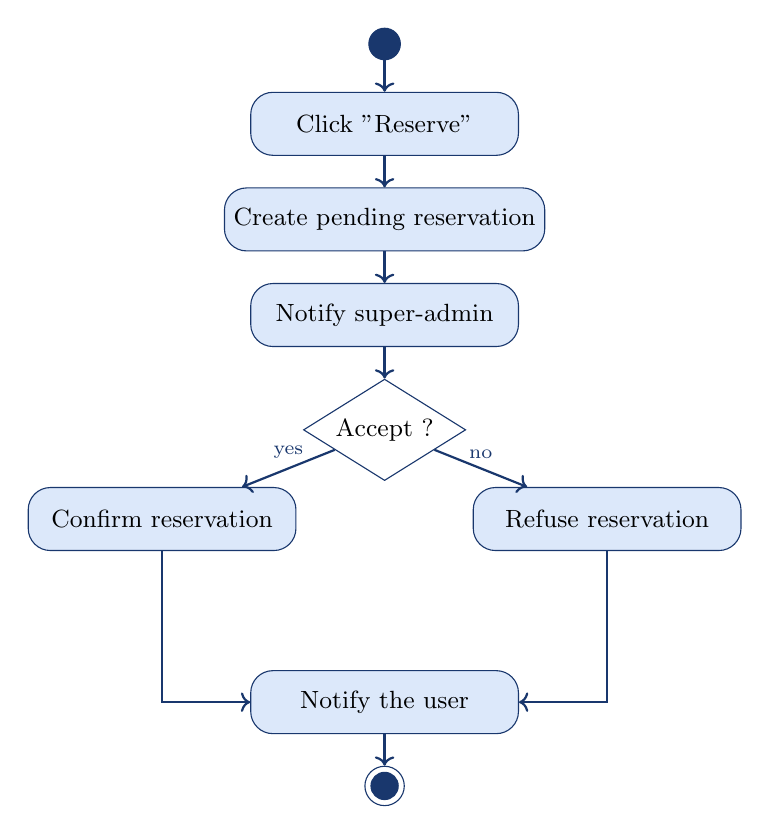
\begin{tikzpicture}[
  every node/.style={font=\small},
  start/.style={circle, draw=primary, fill=primary, minimum size=0.4cm, inner sep=0pt},
  stop/.style={circle, draw=primary, fill=white, minimum size=0.5cm, inner sep=0pt,
               path picture={\fill[primary] (path picture bounding box.center) circle (0.18);}},
  act/.style={rectangle, draw=primary, fill=softblue, rounded corners=8pt,
              minimum width=3.4cm, minimum height=0.8cm, align=center},
  dec/.style={diamond, draw=primary, fill=white, aspect=1.6, align=center, inner sep=2pt},
  arr/.style={->, thick, color=primary}
]
  \node[start] (s) {};
  \node[act, below=0.4cm of s] (a1) {Click "Reserve"};
  \node[act, below=0.4cm of a1] (a2) {Create pending reservation};
  \node[act, below=0.4cm of a2] (a3) {Notify super-admin};
  \node[dec, below=0.4cm of a3] (d) {Accept ?};
  \node[act, below left=0.4cm and 0.6cm of d] (a4) {Confirm reservation};
  \node[act, below right=0.4cm and 0.6cm of d] (a5) {Refuse reservation};
  \node[act, below=2.4cm of d] (a6) {Notify the user};
  \node[stop, below=0.4cm of a6] (e) {};

  \draw[arr] (s) -- (a1);
  \draw[arr] (a1) -- (a2);
  \draw[arr] (a2) -- (a3);
  \draw[arr] (a3) -- (d);
  \draw[arr] (d) -- node[above,font=\scriptsize]{yes} (a4);
  \draw[arr] (d) -- node[above,font=\scriptsize]{no}  (a5);
  \draw[arr] (a4) |- (a6);
  \draw[arr] (a5) |- (a6);
  \draw[arr] (a6) -- (e);
\end{tikzpicture}
\caption{Activity diagram of the reservation workflow}
\label{fig:ad-reservation}
\end{figure}

% ---------- 5.4 sequence ----------
\section{Sequence Diagrams}

\subsection{Sequence : Reserve and notify}

\begin{figure}[H]
\centering
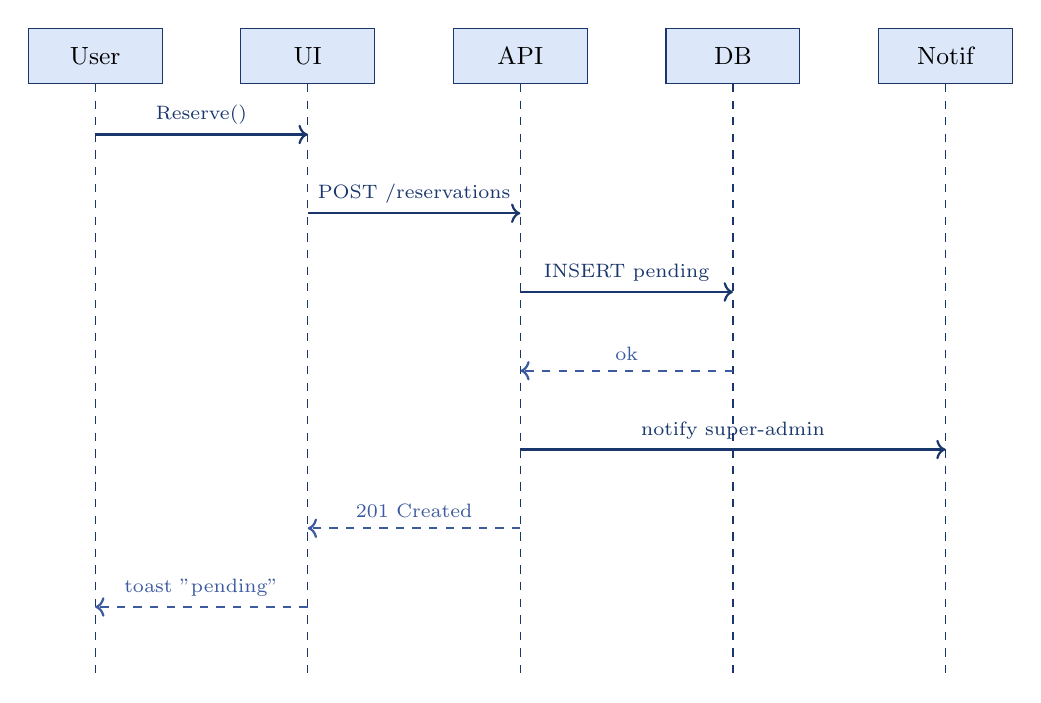
\begin{tikzpicture}[
  every node/.style={font=\small},
  lifeline/.style={dashed, color=primary},
  msg/.style={->, thick, color=primary},
  ret/.style={->, thick, dashed, color=secondary},
  actor/.style={rectangle, draw=primary, fill=softblue, minimum width=1.7cm, minimum height=0.7cm}
]
  \node[actor] (u)  at (0,0)   {User};
  \node[actor] (ui) at (2.7,0) {UI};
  \node[actor] (api)at (5.4,0) {API};
  \node[actor] (db) at (8.1,0) {DB};
  \node[actor] (no) at (10.8,0){Notif};

  \foreach \n in {u,ui,api,db,no} \draw[lifeline] (\n.south) -- ++(0,-7.5);

  \draw[msg] (0,-1)   -- node[above,font=\scriptsize]{Reserve()} (2.7,-1);
  \draw[msg] (2.7,-2) -- node[above,font=\scriptsize]{POST /reservations} (5.4,-2);
  \draw[msg] (5.4,-3) -- node[above,font=\scriptsize]{INSERT pending} (8.1,-3);
  \draw[ret] (8.1,-4) -- node[above,font=\scriptsize]{ok} (5.4,-4);
  \draw[msg] (5.4,-5) -- node[above,font=\scriptsize]{notify super-admin} (10.8,-5);
  \draw[ret] (5.4,-6) -- node[above,font=\scriptsize]{201 Created} (2.7,-6);
  \draw[ret] (2.7,-7) -- node[above,font=\scriptsize]{toast "pending"} (0,-7);
\end{tikzpicture}
\caption{Sequence diagram : Reserve and notify}
\label{fig:sd-reserve}
\end{figure}

% ---------- 5.5 class diagram ----------
\section{Class Diagram of the Module}

\begin{figure}[H]
\centering
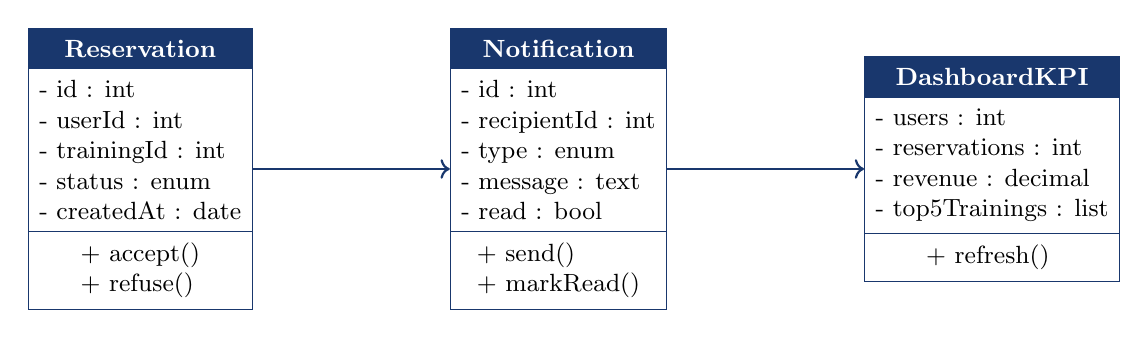
\begin{tikzpicture}[
  every node/.style={font=\small},
  class/.style={rectangle split, rectangle split parts=3,
                rectangle split part fill={primary, white, white},
                draw=primary, text=white, rectangle split draw splits=true, align=left, inner sep=4pt}
]
  \node[class] (res) at (0,0) {%
    \nodepart{one}\bfseries Reservation
    \nodepart[text=black]{two}
      - id : int\\
      - userId : int\\
      - trainingId : int\\
      - status : enum\\
      - createdAt : date
    \nodepart[text=black]{three}
      + accept()\\
      + refuse()
  };

  \node[class, right=2.5cm of res] (notif) {%
    \nodepart{one}\bfseries Notification
    \nodepart[text=black]{two}
      - id : int\\
      - recipientId : int\\
      - type : enum\\
      - message : text\\
      - read : bool
    \nodepart[text=black]{three}
      + send()\\
      + markRead()
  };

  \node[class, right=2.5cm of notif] (kpi) {%
    \nodepart{one}\bfseries DashboardKPI
    \nodepart[text=black]{two}
      - users : int\\
      - reservations : int\\
      - revenue : decimal\\
      - top5Trainings : list
    \nodepart[text=black]{three}
      + refresh()
  };

  \draw[->, thick, color=primary] (res) -- (notif);
  \draw[->, thick, color=primary] (notif) -- (kpi);
\end{tikzpicture}
\caption{Class diagram -- Reservation, Notification \& Dashboard}
\label{fig:cd-r3}
\end{figure}

% ---------- 5.6 dashboard / KPIs ----------
\section{Smart Dashboard \& KPIs}

The smart dashboard, accessible to administrators and the super-administrator, exposes the platform's pulse in real time.

\begin{figure}[H]
\centering
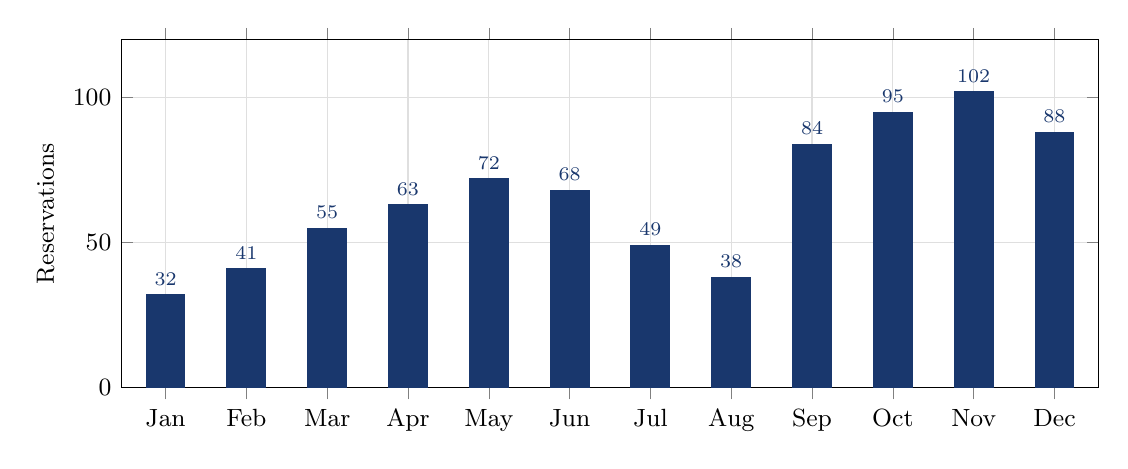
\begin{tikzpicture}
\begin{axis}[
  width=14cm, height=6cm,
  ybar,
  bar width=14pt,
  ylabel={Reservations},
  symbolic x coords={Jan, Feb, Mar, Apr, May, Jun, Jul, Aug, Sep, Oct, Nov, Dec},
  xtick=data,
  ymin=0, ymax=120,
  enlarge x limits=0.05,
  nodes near coords,
  nodes near coords style={font=\scriptsize\bfseries, color=primary},
  every axis label/.append style={font=\small},
  tick label style={font=\small},
  grid=both,
  major grid style={color=gray!25},
  minor grid style={color=gray!10}
]
  \addplot[fill=primary, draw=primary] coordinates {
    (Jan,32) (Feb,41) (Mar,55) (Apr,63) (May,72) (Jun,68)
    (Jul,49) (Aug,38) (Sep,84) (Oct,95) (Nov,102) (Dec,88)
  };
\end{axis}
\end{tikzpicture}
\caption{Monthly reservations over a representative year (sample data)}
\label{fig:kpi-month}
\end{figure}

\begin{figure}[H]
\centering
\begin{tikzpicture}
\begin{axis}[
  width=12cm, height=5.5cm,
  xbar,
  bar width=12pt,
  xlabel={Reservations},
  symbolic y coords={Web Dev, Data Science, Networks, DevOps, Soft Skills},
  ytick=data,
  xmin=0, xmax=140,
  nodes near coords,
  nodes near coords style={font=\small\bfseries, color=primary},
  enlarge y limits=0.18
]
  \addplot[fill=secondary, draw=secondary] coordinates {
    (118, Web Dev) (96, Data Science) (74, Networks) (62, DevOps) (45, Soft Skills)
  };
\end{axis}
\end{tikzpicture}
\caption{Top 5 trainings by reservations (sample data)}
\label{fig:kpi-top5}
\end{figure}

\subsection{Chatbot}

The integrated chatbot answers natural-language queries from the admin (e.g. \textit{"how many reservations this week?"}, \textit{"top 3 trainings"}) by routing them to the dashboard service. It enables a faster decision loop without writing any SQL or navigating multiple pages.

% ---------- 5.7 ----------
\section{Achieved Increment}

\begin{itemize}[leftmargin=2em,itemsep=0.2em]
  \item Full reservation workflow with pending / accepted / refused statuses.
  \item Real-time notifications (in-app + e-mail) for users, admins and super-admin.
  \item Smart dashboard with KPIs, charts and quick filters.
  \item Conversational chatbot that exposes the dashboard in natural language.
  \item Excel/PDF export and Excel import for users and reservations.
\end{itemize}

\section{Conclusion}

With this third release, the ADVANCIA platform reaches its target perimeter. The next chapter steps back from features and looks at the \textit{realization} : the technical environment, the architecture and the most representative interfaces of the final product.
     % Release 3 - Reservation, Notifications & Dashboard
% =============================================================
%  CHAPTER 6 - REALIZATION
% =============================================================

\chapteroverview{Realization}{
  \item Introduction
  \item Hardware Environment
  \item Software Environment
  \item Adopted Architecture
  \item Database Schema
  \item Project Statistics
  \item Representative Interfaces
  \item Tests and Validation
  \item Conclusion
}

\section{Introduction}

After describing \textit{what} the platform does, this last chapter explains \textit{how} it has been built. We present the hardware and software environments, the adopted architecture, the database schema, a few representative interfaces and the validation strategy that supports the quality of the final product.

% ---------- 6.2 hardware ----------
\section{Hardware Environment}

\begin{table}[H]
\centering
\renewcommand{\arraystretch}{1.35}
\begin{tabularx}{\textwidth}{|>{\columncolor{softblue}}l|X|}
\hline
\rowcolor{primary}
\textbf{\color{white} Component} & \textbf{\color{white} Specification}\\
\hline
Processor & Intel Core i5 / i7 (10th generation or higher) \\\hline
RAM       & 8 -- 16 GB DDR4 \\\hline
Storage   & 256 -- 512 GB SSD \\\hline
Display   & 14" -- 15.6" Full HD \\\hline
Network   & Wi-Fi 5 / Wi-Fi 6, Ethernet \\\hline
\end{tabularx}
\caption{Hardware environment used during development}
\label{tab:hw}
\end{table}

% ---------- 6.3 software ----------
\section{Software Environment}

\subsection{Languages and frameworks}

\begin{figure}[H]
\centering
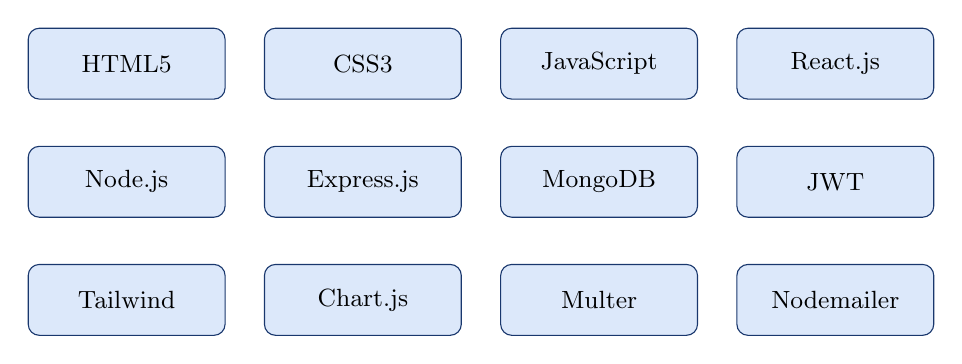
\begin{tikzpicture}[
  every node/.style={font=\small},
  techbox/.style={rectangle, draw=primary, fill=softblue, rounded corners=4pt,
                  minimum width=2.5cm, minimum height=0.9cm, align=center}
]
  \node[techbox] (a) at (0,0)   {HTML5};
  \node[techbox] (b) at (3,0)   {CSS3};
  \node[techbox] (c) at (6,0)   {JavaScript};
  \node[techbox] (d) at (9,0)   {React.js};
  \node[techbox] (e) at (0,-1.5){Node.js};
  \node[techbox] (f) at (3,-1.5){Express.js};
  \node[techbox] (g) at (6,-1.5){MongoDB};
  \node[techbox] (h) at (9,-1.5){JWT};
  \node[techbox] (i) at (0,-3)  {Tailwind};
  \node[techbox] (j) at (3,-3)  {Chart.js};
  \node[techbox] (k) at (6,-3)  {Multer};
  \node[techbox] (l) at (9,-3)  {Nodemailer};
\end{tikzpicture}
\caption{Technical stack of the ADVANCIA platform}
\label{fig:stack}
\end{figure}

\subsection{Tools}

\begin{table}[H]
\centering
\renewcommand{\arraystretch}{1.35}
\begin{tabularx}{\textwidth}{|>{\columncolor{softblue}}l|X|}
\hline
\rowcolor{primary}
\textbf{\color{white} Tool} & \textbf{\color{white} Usage}\\
\hline
Visual Studio Code & Main IDE for front-end and back-end development. \\\hline
Git \& GitHub      & Source-code management and collaboration. \\\hline
Postman            & Manual testing of the REST API. \\\hline
Figma              & UI/UX design and prototyping. \\\hline
Draw.io / StarUML  & UML modeling. \\\hline
Trello / Jira      & Sprint and backlog tracking. \\\hline
MongoDB Compass    & Database visualization. \\\hline
\LaTeX\ (Overleaf) & Writing of the present dissertation. \\\hline
\end{tabularx}
\caption{Tools used during the project}
\label{tab:tools}
\end{table}

% ---------- 6.4 architecture ----------
\section{Adopted Architecture}

The platform follows a classical three-tier architecture, with a clear separation between the presentation layer (React SPA), the business layer (Express REST API) and the data layer (MongoDB).

\begin{figure}[H]
\centering
\begin{tikzpicture}[
  every node/.style={font=\small},
  layer/.style={rectangle, draw=primary, fill=softblue, rounded corners=6pt,
                minimum width=12cm, minimum height=1.6cm, align=center},
  client/.style={rectangle, draw=primary, fill=white, rounded corners=4pt,
                 minimum width=2.5cm, minimum height=0.9cm, align=center},
  arr/.style={->, thick, color=primary}
]
  \node[layer] (l1) at (0,4) {\textbf{Presentation layer}\\React SPA -- Tailwind UI -- Chart.js};
  \node[layer] (l2) at (0,2) {\textbf{Business layer}\\Express REST API -- JWT -- Validation -- Mailer};
  \node[layer] (l3) at (0,0) {\textbf{Data layer}\\MongoDB collections + GridFS for files};

  \draw[arr] (l1) -- node[right]{HTTPS / JSON} (l2);
  \draw[arr] (l2) -- node[right]{Mongoose ORM}  (l3);

  \node[client, left=0.4cm of l1] (cl) {\faDesktop\ Browser};
  \draw[arr] (cl) -- (l1);
\end{tikzpicture}
\caption{Three-tier architecture of the ADVANCIA platform}
\label{fig:arch}
\end{figure}

\subsection{Deployment view}

\begin{figure}[H]
\centering
\begin{tikzpicture}[
  every node/.style={font=\small},
  srv/.style={rectangle, draw=primary, fill=softblue, rounded corners=4pt,
              minimum width=3cm, minimum height=1cm, align=center},
  arr/.style={->, thick, color=primary}
]
  \node[srv] (browser) at (0,0)   {\faDesktop\ Browser};
  \node[srv] (front)   at (4,0)   {\faServer\ Front Server\\(Vite / Nginx)};
  \node[srv] (api)     at (8,0)   {\faCogs\ API Server\\(Node + Express)};
  \node[srv] (db)      at (12,0)  {\faDatabase\ MongoDB};
  \node[srv] (mail)    at (8,-1.8){\faEnvelope\ SMTP / Mail};

  \draw[arr] (browser) -- (front);
  \draw[arr] (front)   -- (api);
  \draw[arr] (api)     -- (db);
  \draw[arr] (api)     -- (mail);
\end{tikzpicture}
\caption{Simplified deployment diagram}
\label{fig:deploy}
\end{figure}

% ---------- 6.5 DB ----------
\section{Database Schema}

\begin{figure}[H]
\centering
\resizebox{\textwidth}{!}{%
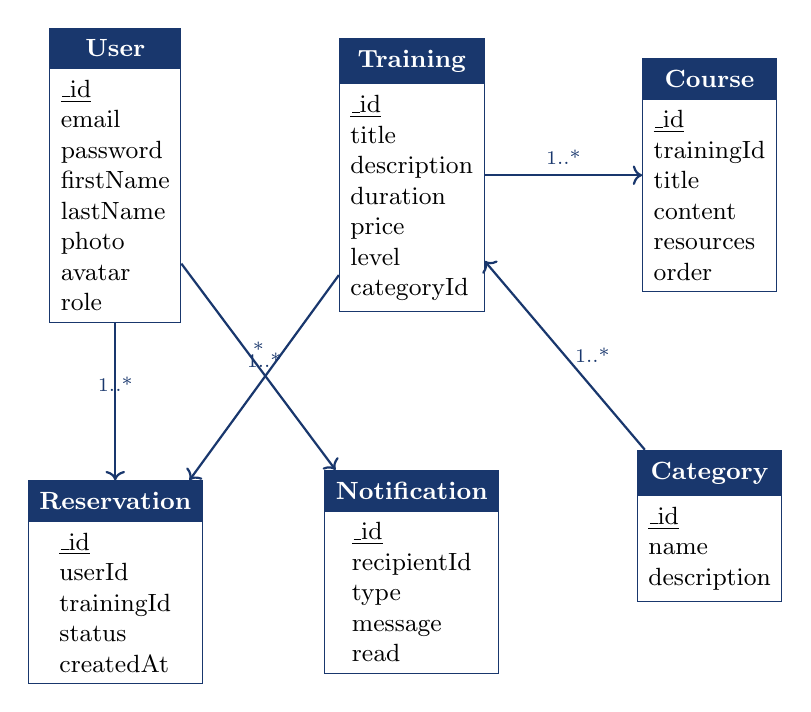
\begin{tikzpicture}[
  every node/.style={font=\small},
  ent/.style={rectangle split, rectangle split parts=2,
              rectangle split part fill={primary, white},
              draw=primary, text=white, rectangle split draw splits=true, align=left, inner sep=4pt}
]
  \node[ent] (u) at (0,0) {%
    \nodepart{one}\bfseries User
    \nodepart[text=black]{two}
      \underline{\_id}\\ email\\ password\\ firstName\\ lastName\\ photo\\ avatar\\ role
  };
  \node[ent, right=2cm of u] (t) {%
    \nodepart{one}\bfseries Training
    \nodepart[text=black]{two}
      \underline{\_id}\\ title\\ description\\ duration\\ price\\ level\\ categoryId
  };
  \node[ent, right=2cm of t] (c) {%
    \nodepart{one}\bfseries Course
    \nodepart[text=black]{two}
      \underline{\_id}\\ trainingId\\ title\\ content\\ resources\\ order
  };
  \node[ent, below=2cm of u] (r) {%
    \nodepart{one}\bfseries Reservation
    \nodepart[text=black]{two}
      \underline{\_id}\\ userId\\ trainingId\\ status\\ createdAt
  };
  \node[ent, below=2cm of t] (n) {%
    \nodepart{one}\bfseries Notification
    \nodepart[text=black]{two}
      \underline{\_id}\\ recipientId\\ type\\ message\\ read
  };
  \node[ent, below=2cm of c] (cat) {%
    \nodepart{one}\bfseries Category
    \nodepart[text=black]{two}
      \underline{\_id}\\ name\\ description
  };

  \draw[->, thick, primary] (u)   -- node[above,font=\scriptsize]{1..*}(r);
  \draw[->, thick, primary] (t)   -- node[above,font=\scriptsize]{1..*}(r);
  \draw[->, thick, primary] (t)   -- node[above,font=\scriptsize]{1..*}(c);
  \draw[->, thick, primary] (cat) -- node[right,font=\scriptsize]{1..*}(t);
  \draw[->, thick, primary] (u)   -- node[above,font=\scriptsize]{*}(n);
\end{tikzpicture}}
\caption{Entity-relationship schema of the ADVANCIA database}
\label{fig:erd}
\end{figure}

% ---------- 6.6 stats ----------
\section{Project Statistics}

\begin{table}[H]
\centering
\renewcommand{\arraystretch}{1.35}
\begin{tabularx}{\textwidth}{|>{\columncolor{softblue}}l|X|}
\hline
\rowcolor{primary}
\textbf{\color{white} Indicator} & \textbf{\color{white} Value}\\
\hline
Number of user stories      & 18 \\\hline
Number of releases          & 3 \\\hline
Number of sprints           & 6 \\\hline
Total story points          & 95 \\\hline
Front-end pages             & $\sim$ 22 \\\hline
REST API endpoints          & $\sim$ 45 \\\hline
Database collections        & 7 \\\hline
Manual test cases           & $\sim$ 60 \\\hline
\end{tabularx}
\caption{Quantitative indicators of the project}
\label{tab:stats}
\end{table}

\subsection{Code distribution}

\begin{figure}[H]
\centering
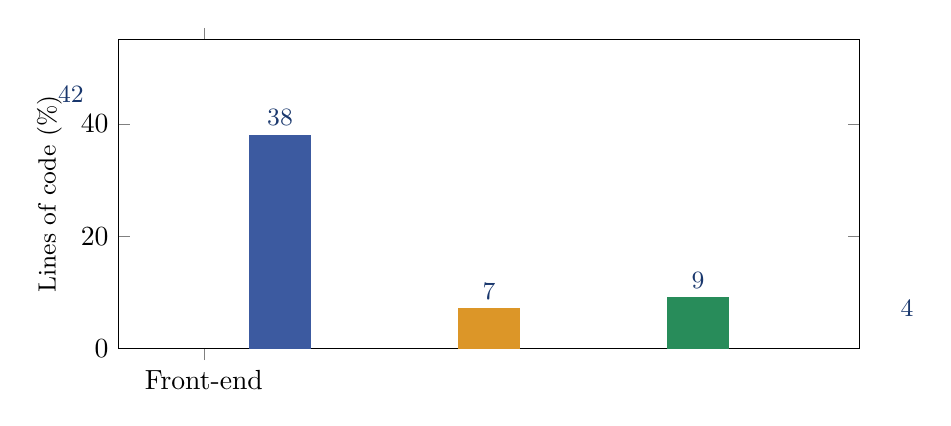
\begin{tikzpicture}
\begin{axis}[
  width=11cm, height=5.5cm,
  ybar,
  bar width=22pt,
  ylabel={Lines of code (\%)},
  symbolic x coords={Front-end, Back-end, Database, Tests, Config},
  xtick=data,
  ymin=0, ymax=55,
  nodes near coords,
  nodes near coords style={font=\small\bfseries, color=primary},
  enlarge x limits=0.15,
  every axis label/.append style={font=\small}
]
  \addplot[fill=primary,    draw=primary]    coordinates {(Front-end,42)};
  \addplot[fill=secondary,  draw=secondary]  coordinates {(Back-end,38)};
  \addplot[fill=accent,     draw=accent]     coordinates {(Database,7)};
  \addplot[fill=success,    draw=success]    coordinates {(Tests,9)};
  \addplot[fill=danger,     draw=danger]     coordinates {(Config,4)};
\end{axis}
\end{tikzpicture}
\caption{Approximate distribution of the code base}
\label{fig:codedist}
\end{figure}

\subsection{Sprint velocity}

\begin{figure}[H]
\centering
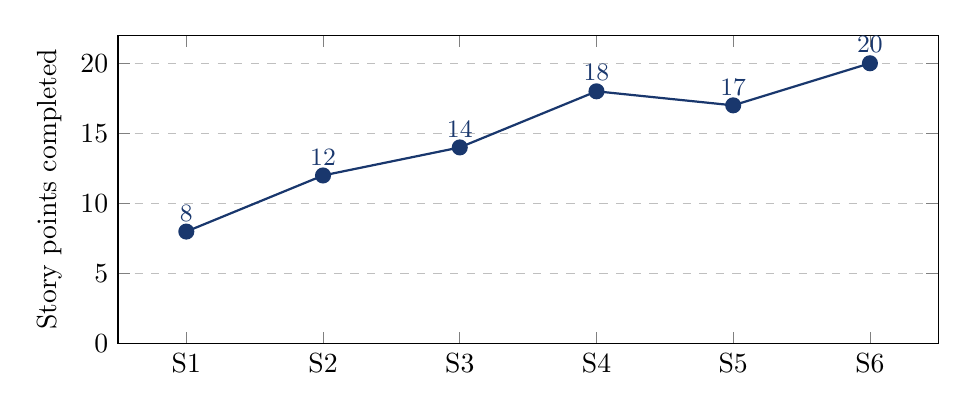
\begin{tikzpicture}
\begin{axis}[
  width=12cm, height=5.5cm,
  ymajorgrids, grid style=dashed,
  ylabel={Story points completed},
  symbolic x coords={S1, S2, S3, S4, S5, S6},
  xtick=data,
  ymin=0, ymax=22,
  mark size=2.5pt,
  nodes near coords,
  nodes near coords style={font=\small\bfseries, color=primary}
]
  \addplot[mark=*, color=primary, thick] coordinates {
    (S1,8) (S2,12) (S3,14) (S4,18) (S5,17) (S6,20)
  };
\end{axis}
\end{tikzpicture}
\caption{Velocity per sprint (story points completed)}
\label{fig:velocity}
\end{figure}

% ---------- 6.7 screens ----------
\section{Representative Interfaces}

This section illustrates the main interfaces produced. Real screenshots will replace the placeholders in the final printed version of the dissertation.

\begin{figure}[H]
\centering
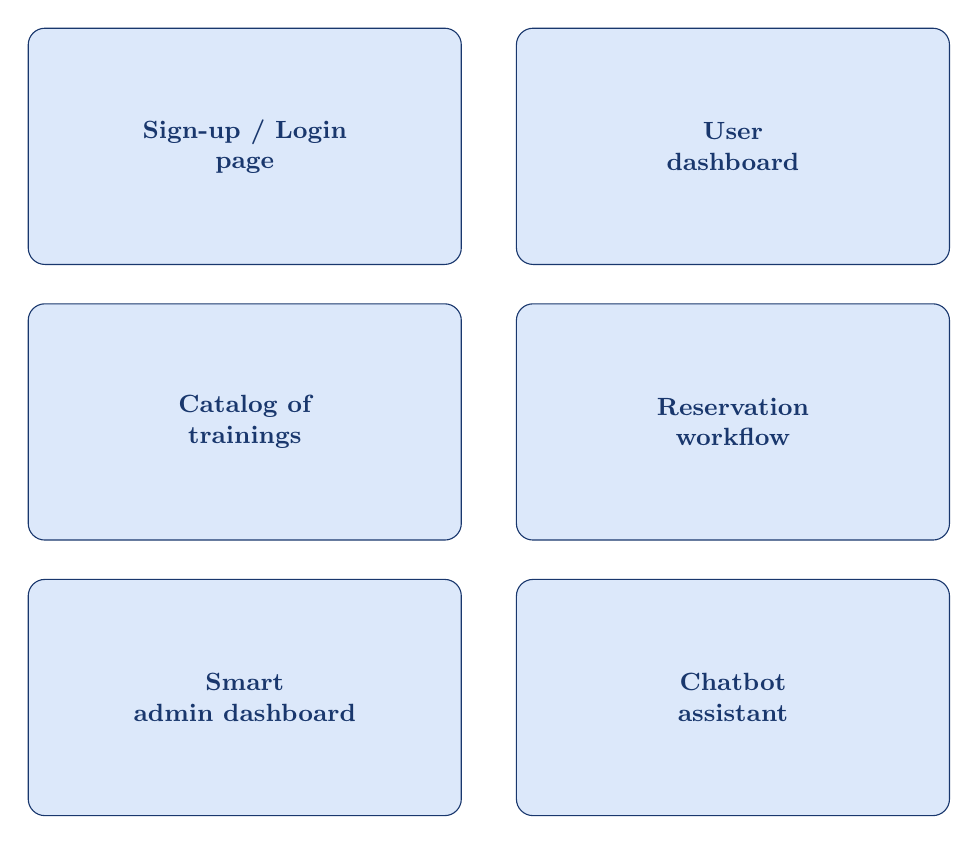
\begin{tikzpicture}[
  every node/.style={font=\small},
  scr/.style={rectangle, draw=primary, fill=softblue, rounded corners=6pt,
              minimum width=5.5cm, minimum height=3cm, align=center,
              font=\small\bfseries\color{primary}}
]
  \node[scr] (a) at (0,0)   {Sign-up / Login\\page};
  \node[scr] (b) at (6.2,0) {User\\dashboard};
  \node[scr] (c) at (0,-3.5){Catalog of\\trainings};
  \node[scr] (d) at (6.2,-3.5){Reservation\\workflow};
  \node[scr] (e) at (0,-7)  {Smart\\admin dashboard};
  \node[scr] (f) at (6.2,-7){Chatbot\\assistant};
\end{tikzpicture}
\caption{Mosaic of the main interfaces of the platform}
\label{fig:mosaic}
\end{figure}

% ---------- 6.8 tests ----------
\section{Tests and Validation}

A pyramid testing strategy was followed during the project : unit tests at the bottom (most numerous, fastest), integration tests in the middle, and end-to-end tests at the top (less numerous, slower but representative of the user journey).

\begin{figure}[H]
\centering
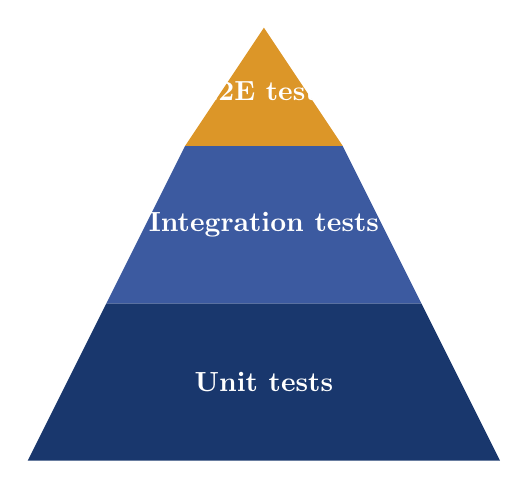
\begin{tikzpicture}
  \fill[primary]   (-3,0) -- (3,0)  -- (2,2) -- (-2,2) -- cycle;
  \fill[secondary] (-2,2) -- (2,2)  -- (1,4) -- (-1,4) -- cycle;
  \fill[accent]    (-1,4) -- (1,4)  -- (0,5.5) -- cycle;

  \node[white, font=\bfseries] at (0,1)   {Unit tests};
  \node[white, font=\bfseries] at (0,3)   {Integration tests};
  \node[white, font=\bfseries] at (0,4.7) {E2E tests};
\end{tikzpicture}
\caption{Testing pyramid adopted}
\label{fig:pyramid}
\end{figure}

\begin{table}[H]
\centering
\renewcommand{\arraystretch}{1.35}
\begin{tabularx}{\textwidth}{|>{\columncolor{softblue}}l|c|c|X|}
\hline
\rowcolor{primary}
\textbf{\color{white} Test} & \textbf{\color{white} Cases} & \textbf{\color{white} Pass rate} & \textbf{\color{white} Coverage}\\
\hline
Unit (services)      & 38 & 100 \% & Auth, reservation, dashboard \\\hline
Integration (API)    & 16 & 100 \% & Critical endpoints \\\hline
E2E (UI)             & 8  & 100 \% & Sign-up, reserve, accept, export \\\hline
\end{tabularx}
\caption{Synthesis of the validation tests}
\label{tab:tests}
\end{table}

\section{Conclusion}

This realization chapter has materialized the project on a technical level : a modern stack, a clean three-tier architecture, a documented database, measurable indicators and a structured testing strategy. The platform is now ready for delivery and for the perspectives of evolution detailed in the general conclusion.
     % Realisation (technical environment & screens)

% ---------- GENERAL CONCLUSION ----------
% =============================================================
%  GENERAL CONCLUSION
% =============================================================

\chapter*{General Conclusion}
\addcontentsline{toc}{chapter}{General Conclusion}
\markboth{General Conclusion}{}

\setstretch{1.5}

\noindent
The journey we have just described is, at its heart, the story of a problem turned into a solution. Faced with a daily reality where reservations, user records, communications and reports were scattered across paper, spreadsheets and phone calls, our mission was to bring them together inside a single, modern and intelligent web platform : \textbf{ADVANCIA}.

\medskip
\noindent
Throughout this dissertation, we have followed a clear thread. The \textit{first chapter} settled the framework of the project : the host company \textsc{ADVANCIA Training Center}, the limitations of the existing solutions and the chosen agile process. The \textit{second chapter} translated the need into a precise plan -- four actors, eighteen user stories, three releases and a Gantt schedule. \textit{Chapters three to five} delivered the platform, sprint after sprint : authentication and user management, training catalog and course management, then reservations, notifications, smart dashboard and chatbot. The \textit{sixth chapter} closed the loop by anchoring the product on a clean technical environment and a measured quality strategy.

\medskip
\noindent
The result is a coherent platform, validated against its initial objectives :

\begin{itemize}[leftmargin=2.2em,itemsep=0.4em]
  \item A \textbf{secure identity layer} based on JWT and role-based access control.
  \item A \textbf{four-actor model} -- User, Trainer, Admin, Super-Admin -- each with a tailored experience.
  \item A \textbf{complete reservation workflow}, from request to acceptance, with traceable status transitions.
  \item A \textbf{smart dashboard} backed by real KPIs and supported by an integrated \textbf{chatbot}.
  \item A \textbf{multi-format data exchange} (Excel \& PDF), aligned with the daily operations of the company.
\end{itemize}

\medskip
\noindent
On a personal level, this project has been far more than a development exercise. It taught us how to listen to a real client, how to translate fuzzy expectations into precise stories, how to defend technical choices and how to deliver value in short, measurable cycles. It also reinforced our conviction that \textit{good software is, first and foremost, a faithful answer to a human need}.

\medskip
\noindent
\textbf{Perspectives.} Several evolutions can naturally extend the present work :

\begin{itemize}[leftmargin=2.2em,itemsep=0.3em]
  \item A \textbf{native mobile application} (React Native / Flutter) reusing the existing REST API.
  \item An \textbf{AI-assisted recommendation engine} suggesting personalized trainings to each user.
  \item An \textbf{online payment} module to close the reservation cycle end-to-end.
  \item A more advanced \textbf{learning analytics} layer for trainers (engagement, completion, retention).
  \item A \textbf{multilingual interface} (Arabic / French / English) to broaden the audience.
\end{itemize}

\medskip
\noindent
We hope that \textbf{ADVANCIA} will, beyond this dissertation, find its place as a useful tool for its users and as a stepping stone for the future engineers who will continue to extend it.

\cleardoublepage


% ---------- NETOGRAPHY ----------
% =============================================================
%  NETOGRAPHY
% =============================================================

\chapter*{Netography}
\addcontentsline{toc}{chapter}{Netography}
\markboth{Netography}{}

\setstretch{1.4}

\begin{enumerate}[leftmargin=2em,itemsep=0.4em]
  \item React.js -- Official Documentation. \\
        \url{https://react.dev/} -- Last access : April 2026.
  \item Node.js -- Official Documentation. \\
        \url{https://nodejs.org/en/docs} -- Last access : April 2026.
  \item Express.js -- Web framework for Node.js. \\
        \url{https://expressjs.com/} -- Last access : April 2026.
  \item MongoDB -- Database documentation. \\
        \url{https://www.mongodb.com/docs/} -- Last access : April 2026.
  \item Mongoose -- ODM for MongoDB. \\
        \url{https://mongoosejs.com/docs/guide.html} -- Last access : April 2026.
  \item JWT -- Introduction to JSON Web Tokens. \\
        \url{https://jwt.io/introduction} -- Last access : April 2026.
  \item Tailwind CSS -- Utility-first CSS framework. \\
        \url{https://tailwindcss.com/docs} -- Last access : April 2026.
  \item Chart.js -- Open-source charting library. \\
        \url{https://www.chartjs.org/docs/latest/} -- Last access : April 2026.
  \item Multer -- Node.js middleware for file uploads. \\
        \url{https://github.com/expressjs/multer} -- Last access : April 2026.
  \item Nodemailer -- E-mail sending for Node.js. \\
        \url{https://nodemailer.com/} -- Last access : April 2026.
  \item Postman -- API testing tool. \\
        \url{https://www.postman.com/} -- Last access : April 2026.
  \item Figma -- UI/UX design platform. \\
        \url{https://www.figma.com/} -- Last access : April 2026.
  \item Scrum Guide -- Official Scrum framework guide. \\
        \url{https://scrumguides.org/} -- Last access : April 2026.
  \item ISET Siliana -- Official website. \\
        \url{https://www.iset-siliana.rnu.tn/} -- Last access : April 2026.
  \item ADVANCIA Training Center -- Official website. \\
        \url{https://www.advancia-tc.com/} -- Last access : April 2026.
\end{enumerate}

\cleardoublepage


\end{document}
